\documentclass[twoside]{book}

% Packages required by doxygen
\usepackage{fixltx2e}
\usepackage{calc}
\usepackage{doxygen}
\usepackage[export]{adjustbox} % also loads graphicx
\usepackage{graphicx}
\usepackage[utf8]{inputenc}
\usepackage{makeidx}
\usepackage{multicol}
\usepackage{multirow}
\PassOptionsToPackage{warn}{textcomp}
\usepackage{textcomp}
\usepackage[nointegrals]{wasysym}
\usepackage[table]{xcolor}

% NLS support packages
\usepackage[french]{babel}
\NoAutoSpaceBeforeFDP

% Font selection
\usepackage[T1]{fontenc}
\usepackage[scaled=.90]{helvet}
\usepackage{courier}
\usepackage{amssymb}
\usepackage{sectsty}
\renewcommand{\familydefault}{\sfdefault}
\allsectionsfont{%
  \fontseries{bc}\selectfont%
  \color{darkgray}%
}
\renewcommand{\DoxyLabelFont}{%
  \fontseries{bc}\selectfont%
  \color{darkgray}%
}
\newcommand{\+}{\discretionary{\mbox{\scriptsize$\hookleftarrow$}}{}{}}

% Page & text layout
\usepackage{geometry}
\geometry{%
  a4paper,%
  top=2.5cm,%
  bottom=2.5cm,%
  left=2.5cm,%
  right=2.5cm%
}
\tolerance=750
\hfuzz=15pt
\hbadness=750
\setlength{\emergencystretch}{15pt}
\setlength{\parindent}{0cm}
\setlength{\parskip}{3ex plus 2ex minus 2ex}
\makeatletter
\renewcommand{\paragraph}{%
  \@startsection{paragraph}{4}{0ex}{-1.0ex}{1.0ex}{%
    \normalfont\normalsize\bfseries\SS@parafont%
  }%
}
\renewcommand{\subparagraph}{%
  \@startsection{subparagraph}{5}{0ex}{-1.0ex}{1.0ex}{%
    \normalfont\normalsize\bfseries\SS@subparafont%
  }%
}
\makeatother

% Headers & footers
\usepackage{fancyhdr}
\pagestyle{fancyplain}
\fancyhead[LE]{\fancyplain{}{\bfseries\thepage}}
\fancyhead[CE]{\fancyplain{}{}}
\fancyhead[RE]{\fancyplain{}{\bfseries\leftmark}}
\fancyhead[LO]{\fancyplain{}{\bfseries\rightmark}}
\fancyhead[CO]{\fancyplain{}{}}
\fancyhead[RO]{\fancyplain{}{\bfseries\thepage}}
\fancyfoot[LE]{\fancyplain{}{}}
\fancyfoot[CE]{\fancyplain{}{}}
\fancyfoot[RE]{\fancyplain{}{\bfseries\scriptsize Généré par Doxygen }}
\fancyfoot[LO]{\fancyplain{}{\bfseries\scriptsize Généré par Doxygen }}
\fancyfoot[CO]{\fancyplain{}{}}
\fancyfoot[RO]{\fancyplain{}{}}
\renewcommand{\footrulewidth}{0.4pt}
\renewcommand{\chaptermark}[1]{%
  \markboth{#1}{}%
}
\renewcommand{\sectionmark}[1]{%
  \markright{\thesection\ #1}%
}

% Indices & bibliography
\usepackage{natbib}
\usepackage[titles]{tocloft}
\setcounter{tocdepth}{3}
\setcounter{secnumdepth}{5}
\makeindex

% Hyperlinks (required, but should be loaded last)
\usepackage{ifpdf}
\ifpdf
  \usepackage[pdftex,pagebackref=true]{hyperref}
\else
  \usepackage[ps2pdf,pagebackref=true]{hyperref}
\fi
\hypersetup{%
  colorlinks=true,%
  linkcolor=blue,%
  citecolor=blue,%
  unicode%
}

% Custom commands
\newcommand{\clearemptydoublepage}{%
  \newpage{\pagestyle{empty}\cleardoublepage}%
}

\usepackage{caption}
\captionsetup{labelsep=space,justification=centering,font={bf},singlelinecheck=off,skip=4pt,position=top}

%===== C O N T E N T S =====

\begin{document}

% Titlepage & ToC
\hypersetup{pageanchor=false,
             bookmarksnumbered=true,
             pdfencoding=unicode
            }
\pagenumbering{alph}
\begin{titlepage}
\vspace*{7cm}
\begin{center}%
{\Large Drones }\\
\vspace*{1cm}
{\large Généré par Doxygen 1.8.14}\\
\end{center}
\end{titlepage}
\clearemptydoublepage
\pagenumbering{roman}
\tableofcontents
\clearemptydoublepage
\pagenumbering{arabic}
\hypersetup{pageanchor=true}

%--- Begin generated contents ---
\chapter{Index hiérarchique}
\section{Hiérarchie des classes}
Cette liste d\textquotesingle{}héritage est classée approximativement par ordre alphabétique \+:\begin{DoxyCompactList}
\item \contentsline{section}{Affichage}{\pageref{class_affichage}}{}
\item \contentsline{section}{Capteur}{\pageref{class_capteur}}{}
\item \contentsline{section}{Comportement}{\pageref{class_comportement}}{}
\begin{DoxyCompactList}
\item \contentsline{section}{Dlite}{\pageref{class_dlite}}{}
\item \contentsline{section}{Naif}{\pageref{class_naif}}{}
\end{DoxyCompactList}
\item \contentsline{section}{Drone}{\pageref{class_drone}}{}
\item \contentsline{section}{Environnement}{\pageref{class_environnement}}{}
\item \contentsline{section}{Essaim}{\pageref{class_essaim}}{}
\item \contentsline{section}{Formation}{\pageref{class_formation}}{}
\begin{DoxyCompactList}
\item \contentsline{section}{Cubique}{\pageref{class_cubique}}{}
\item \contentsline{section}{Pyramidale}{\pageref{class_pyramidale}}{}
\end{DoxyCompactList}
\item \contentsline{section}{Obstacle}{\pageref{class_obstacle}}{}
\item Test\+Fixture\begin{DoxyCompactList}
\item \contentsline{section}{tests\+Capteur}{\pageref{classtests_capteur}}{}
\item \contentsline{section}{tests\+Drone}{\pageref{classtests_drone}}{}
\item \contentsline{section}{tests\+Essaim}{\pageref{classtests_essaim}}{}
\item \contentsline{section}{tests\+Vecteur\+R3}{\pageref{classtests_vecteur_r3}}{}
\end{DoxyCompactList}
\item \contentsline{section}{tests\+Environnement}{\pageref{classtests_environnement}}{}
\item \contentsline{section}{Track\+Ball\+Camera}{\pageref{class_track_ball_camera}}{}
\item \contentsline{section}{Vecteur\+R3}{\pageref{class_vecteur_r3}}{}
\end{DoxyCompactList}

\chapter{Index des classes}
\section{Liste des classes}
Liste des classes, structures, unions et interfaces avec une brève description \+:\begin{DoxyCompactList}
\item\contentsline{section}{\mbox{\hyperlink{class_affichage}{Affichage}} }{\pageref{class_affichage}}{}
\item\contentsline{section}{\mbox{\hyperlink{class_capteur}{Capteur}} }{\pageref{class_capteur}}{}
\item\contentsline{section}{\mbox{\hyperlink{class_comportement}{Comportement}} }{\pageref{class_comportement}}{}
\item\contentsline{section}{\mbox{\hyperlink{class_cubique}{Cubique}} }{\pageref{class_cubique}}{}
\item\contentsline{section}{\mbox{\hyperlink{class_dlite}{Dlite}} }{\pageref{class_dlite}}{}
\item\contentsline{section}{\mbox{\hyperlink{class_drone}{Drone}} }{\pageref{class_drone}}{}
\item\contentsline{section}{\mbox{\hyperlink{class_environnement}{Environnement}} }{\pageref{class_environnement}}{}
\item\contentsline{section}{\mbox{\hyperlink{class_essaim}{Essaim}} }{\pageref{class_essaim}}{}
\item\contentsline{section}{\mbox{\hyperlink{class_formation}{Formation}} }{\pageref{class_formation}}{}
\item\contentsline{section}{\mbox{\hyperlink{class_naif}{Naif}} }{\pageref{class_naif}}{}
\item\contentsline{section}{\mbox{\hyperlink{class_obstacle}{Obstacle}} }{\pageref{class_obstacle}}{}
\item\contentsline{section}{\mbox{\hyperlink{class_pyramidale}{Pyramidale}} }{\pageref{class_pyramidale}}{}
\item\contentsline{section}{\mbox{\hyperlink{classtests_capteur}{tests\+Capteur}} }{\pageref{classtests_capteur}}{}
\item\contentsline{section}{\mbox{\hyperlink{classtests_drone}{tests\+Drone}} }{\pageref{classtests_drone}}{}
\item\contentsline{section}{\mbox{\hyperlink{classtests_environnement}{tests\+Environnement}} }{\pageref{classtests_environnement}}{}
\item\contentsline{section}{\mbox{\hyperlink{classtests_essaim}{tests\+Essaim}} }{\pageref{classtests_essaim}}{}
\item\contentsline{section}{\mbox{\hyperlink{classtests_vecteur_r3}{tests\+Vecteur\+R3}} }{\pageref{classtests_vecteur_r3}}{}
\item\contentsline{section}{\mbox{\hyperlink{class_track_ball_camera}{Track\+Ball\+Camera}} }{\pageref{class_track_ball_camera}}{}
\item\contentsline{section}{\mbox{\hyperlink{class_vecteur_r3}{Vecteur\+R3}} }{\pageref{class_vecteur_r3}}{}
\end{DoxyCompactList}

\chapter{Index des fichiers}
\section{Liste des fichiers}
Liste de tous les fichiers documentés avec une brève description \+:\begin{DoxyCompactList}
\item\contentsline{section}{{\bfseries Affichage.\+h} }{\pageref{_affichage_8h}}{}
\item\contentsline{section}{{\bfseries Capteur.\+h} }{\pageref{_capteur_8h}}{}
\item\contentsline{section}{{\bfseries Comportement.\+h} }{\pageref{_comportement_8h}}{}
\item\contentsline{section}{{\bfseries Cubique.\+h} }{\pageref{_cubique_8h}}{}
\item\contentsline{section}{{\bfseries Dlite.\+h} }{\pageref{_dlite_8h}}{}
\item\contentsline{section}{{\bfseries Drone.\+h} }{\pageref{_drone_8h}}{}
\item\contentsline{section}{{\bfseries Environnement.\+h} }{\pageref{_environnement_8h}}{}
\item\contentsline{section}{{\bfseries Essaim.\+h} }{\pageref{_essaim_8h}}{}
\item\contentsline{section}{{\bfseries Formation.\+h} }{\pageref{_formation_8h}}{}
\item\contentsline{section}{\mbox{\hyperlink{main_8cpp}{main.\+cpp}} }{\pageref{main_8cpp}}{}
\item\contentsline{section}{{\bfseries Naif.\+h} }{\pageref{_naif_8h}}{}
\item\contentsline{section}{{\bfseries Obstacle.\+h} }{\pageref{_obstacle_8h}}{}
\item\contentsline{section}{{\bfseries Pyramidale.\+h} }{\pageref{_pyramidale_8h}}{}
\item\contentsline{section}{{\bfseries sdlglutils.\+h} }{\pageref{sdlglutils_8h}}{}
\item\contentsline{section}{{\bfseries tests\+Capteur.\+h} }{\pageref{tests_capteur_8h}}{}
\item\contentsline{section}{{\bfseries tests\+Comportement.\+h} }{\pageref{tests_comportement_8h}}{}
\item\contentsline{section}{{\bfseries tests\+Cubique.\+h} }{\pageref{tests_cubique_8h}}{}
\item\contentsline{section}{{\bfseries tests\+Drone.\+h} }{\pageref{tests_drone_8h}}{}
\item\contentsline{section}{{\bfseries tests\+Environnement.\+h} }{\pageref{tests_environnement_8h}}{}
\item\contentsline{section}{{\bfseries tests\+Essaim.\+h} }{\pageref{tests_essaim_8h}}{}
\item\contentsline{section}{{\bfseries tests\+Vecteur\+R3.\+h} }{\pageref{tests_vecteur_r3_8h}}{}
\item\contentsline{section}{{\bfseries trackballcamera.\+h} }{\pageref{trackballcamera_8h}}{}
\item\contentsline{section}{{\bfseries Vecteur\+R3.\+h} }{\pageref{_vecteur_r3_8h}}{}
\end{DoxyCompactList}

\chapter{Documentation des classes}
\hypertarget{class_affichage}{}\section{Référence de la classe Affichage}
\label{class_affichage}\index{Affichage@{Affichage}}


{\ttfamily \#include $<$Affichage.\+h$>$}

\subsection*{Fonctions membres publiques}
\begin{DoxyCompactItemize}
\item 
\mbox{\hyperlink{class_affichage_a1e4cd468a67bff4ddc15d3d245188651}{Affichage}} (\mbox{\hyperlink{class_environnement}{Environnement}} $\ast$env)
\item 
virtual \mbox{\hyperlink{class_affichage_ae6a4f4db7a0d8d2abc8bd44c1be674c0}{$\sim$\+Affichage}} ()
\item 
void \mbox{\hyperlink{class_affichage_af90570851774c1f36d53ed10fb016f47}{draw}} (\mbox{\hyperlink{class_track_ball_camera}{Track\+Ball\+Camera}} $\ast$, G\+Luint)
\end{DoxyCompactItemize}


\subsection{Description détaillée}
Classe qui permet d\textquotesingle{}afficher en 3D l\textquotesingle{}\mbox{\hyperlink{class_environnement}{Environnement}}. Cela inclut principalement les Drones et les Obstacles. Utilise open\+GL et S\+DL \begin{DoxyAuthor}{Auteurs}
Timothé, Simon 
\end{DoxyAuthor}


\subsection{Documentation des constructeurs et destructeur}
\mbox{\Hypertarget{class_affichage_a1e4cd468a67bff4ddc15d3d245188651}\label{class_affichage_a1e4cd468a67bff4ddc15d3d245188651}} 
\index{Affichage@{Affichage}!Affichage@{Affichage}}
\index{Affichage@{Affichage}!Affichage@{Affichage}}
\subsubsection{\texorpdfstring{Affichage()}{Affichage()}}
{\footnotesize\ttfamily Affichage\+::\+Affichage (\begin{DoxyParamCaption}\item[{\mbox{\hyperlink{class_environnement}{Environnement}} $\ast$}]{env }\end{DoxyParamCaption})}

Un constructeur utilisant un environnement pour s\textquotesingle{}y lier par pointeur. initialise aussi la texture des drones directement par une valeur donnée dans le constructeur. 
\begin{DoxyParams}{Paramètres}
{\em env} & l\textquotesingle{}\mbox{\hyperlink{class_environnement}{Environnement}} vers lequel pointer; sur lequel \mbox{\hyperlink{class_affichage}{Affichage}} devra faire son travail. \\
\hline
\end{DoxyParams}
\mbox{\Hypertarget{class_affichage_ae6a4f4db7a0d8d2abc8bd44c1be674c0}\label{class_affichage_ae6a4f4db7a0d8d2abc8bd44c1be674c0}} 
\index{Affichage@{Affichage}!````~Affichage@{$\sim$\+Affichage}}
\index{````~Affichage@{$\sim$\+Affichage}!Affichage@{Affichage}}
\subsubsection{\texorpdfstring{$\sim$\+Affichage()}{~Affichage()}}
{\footnotesize\ttfamily Affichage\+::$\sim$\+Affichage (\begin{DoxyParamCaption}{ }\end{DoxyParamCaption})\hspace{0.3cm}{\ttfamily [virtual]}}

Simple Destructeur de l\textquotesingle{}\mbox{\hyperlink{class_affichage}{Affichage}}. 

\subsection{Documentation des fonctions membres}
\mbox{\Hypertarget{class_affichage_af90570851774c1f36d53ed10fb016f47}\label{class_affichage_af90570851774c1f36d53ed10fb016f47}} 
\index{Affichage@{Affichage}!draw@{draw}}
\index{draw@{draw}!Affichage@{Affichage}}
\subsubsection{\texorpdfstring{draw()}{draw()}}
{\footnotesize\ttfamily void Affichage\+::draw (\begin{DoxyParamCaption}\item[{\mbox{\hyperlink{class_track_ball_camera}{Track\+Ball\+Camera}} $\ast$}]{camera,  }\item[{G\+Luint}]{drone\+Text }\end{DoxyParamCaption})}

Méthode principale, affichant l\textquotesingle{}\mbox{\hyperlink{class_environnement}{Environnement}} en attribut 

La documentation de cette classe a été générée à partir des fichiers suivants \+:\begin{DoxyCompactItemize}
\item 
Affichage.\+h\item 
Affichage.\+cpp\end{DoxyCompactItemize}

\hypertarget{class_capteur}{}\section{Référence de la classe Capteur}
\label{class_capteur}\index{Capteur@{Capteur}}


{\ttfamily \#include $<$Capteur.\+h$>$}

\subsection*{Fonctions membres publiques}
\begin{DoxyCompactItemize}
\item 
\mbox{\hyperlink{class_capteur_a507682442d44b555477ada24146be12f}{Capteur}} (const float \&p, const \mbox{\hyperlink{class_vecteur_r3}{Vecteur\+R3}} \&dir, \mbox{\hyperlink{class_environnement}{Environnement}} $\ast$environnement)
\item 
virtual \mbox{\hyperlink{class_capteur_a2bbfecdceba5e9a13fc7c55cc5f7eae3}{$\sim$\+Capteur}} ()
\item 
float \mbox{\hyperlink{class_capteur_a7b56d66e80c4de6c796b32bc978475e9}{get\+Distance\+Detectee}} () const
\item 
float \mbox{\hyperlink{class_capteur_a6022e941e6ebe7d3472a28802ef0b4c0}{get\+Portee}} () const
\item 
\mbox{\Hypertarget{class_capteur_ac37318cd8a0199f42321381f6002aa8f}\label{class_capteur_ac37318cd8a0199f42321381f6002aa8f}} 
void {\bfseries update\+Distance\+Detectee\+Obstacle} ()
\item 
\mbox{\Hypertarget{class_capteur_a4abe39065d4aa28aa457f41424a449af}\label{class_capteur_a4abe39065d4aa28aa457f41424a449af}} 
void {\bfseries update\+Distance\+Detectee\+Bords} ()
\item 
void \mbox{\hyperlink{class_capteur_a0e4afe7bdc6e27985564cf69daedca07}{update\+Distance\+Detectee}} ()
\item 
\mbox{\hyperlink{class_vecteur_r3}{Vecteur\+R3}} \mbox{\hyperlink{class_capteur_aa92b7552969206047df939d641cfb802}{get\+Direction}} () const
\item 
bool \mbox{\hyperlink{class_capteur_a0229c6b8fc7838932c53157eb3110b5b}{detecte\+Q\+Qch}} () const
\item 
void \mbox{\hyperlink{class_capteur_aa25dc5f9211e43691bd8351265a2b3b3}{associer\+Info\+Drone}} (const float, \mbox{\hyperlink{class_vecteur_r3}{Vecteur\+R3}} $\ast$)
\end{DoxyCompactItemize}


\subsection{Description détaillée}
\begin{DoxyAuthor}{Auteurs}
Timothé 
\end{DoxyAuthor}
\begin{DoxyDate}{Date}
20 Avril 2018
\end{DoxyDate}
Les capteurs sont les outils nécéssaires aux drones pour detecter les obstacles alentours à une distance donnée. 

\subsection{Documentation des constructeurs et destructeur}
\mbox{\Hypertarget{class_capteur_a507682442d44b555477ada24146be12f}\label{class_capteur_a507682442d44b555477ada24146be12f}} 
\index{Capteur@{Capteur}!Capteur@{Capteur}}
\index{Capteur@{Capteur}!Capteur@{Capteur}}
\subsubsection{\texorpdfstring{Capteur()}{Capteur()}}
{\footnotesize\ttfamily Capteur\+::\+Capteur (\begin{DoxyParamCaption}\item[{const float \&}]{p,  }\item[{const \mbox{\hyperlink{class_vecteur_r3}{Vecteur\+R3}} \&}]{dir,  }\item[{\mbox{\hyperlink{class_environnement}{Environnement}} $\ast$}]{environnement }\end{DoxyParamCaption})}

Constructeur de \mbox{\hyperlink{class_capteur}{Capteur}} initialisant tous ses paramètres à des valeurs données en entrée. \mbox{\Hypertarget{class_capteur_a2bbfecdceba5e9a13fc7c55cc5f7eae3}\label{class_capteur_a2bbfecdceba5e9a13fc7c55cc5f7eae3}} 
\index{Capteur@{Capteur}!````~Capteur@{$\sim$\+Capteur}}
\index{````~Capteur@{$\sim$\+Capteur}!Capteur@{Capteur}}
\subsubsection{\texorpdfstring{$\sim$\+Capteur()}{~Capteur()}}
{\footnotesize\ttfamily Capteur\+::$\sim$\+Capteur (\begin{DoxyParamCaption}{ }\end{DoxyParamCaption})\hspace{0.3cm}{\ttfamily [virtual]}}

Déstructeur de \mbox{\hyperlink{class_capteur}{Capteur}} 

\subsection{Documentation des fonctions membres}
\mbox{\Hypertarget{class_capteur_aa25dc5f9211e43691bd8351265a2b3b3}\label{class_capteur_aa25dc5f9211e43691bd8351265a2b3b3}} 
\index{Capteur@{Capteur}!associer\+Info\+Drone@{associer\+Info\+Drone}}
\index{associer\+Info\+Drone@{associer\+Info\+Drone}!Capteur@{Capteur}}
\subsubsection{\texorpdfstring{associer\+Info\+Drone()}{associerInfoDrone()}}
{\footnotesize\ttfamily void Capteur\+::associer\+Info\+Drone (\begin{DoxyParamCaption}\item[{const float}]{rayon,  }\item[{\mbox{\hyperlink{class_vecteur_r3}{Vecteur\+R3}} $\ast$}]{\+\_\+p\+Position\+Drone }\end{DoxyParamCaption})}

Associe les informations (utiles au \mbox{\hyperlink{class_capteur}{Capteur}}) du \mbox{\hyperlink{class_drone}{Drone}} à ce \mbox{\hyperlink{class_capteur}{Capteur}} \mbox{\Hypertarget{class_capteur_a0229c6b8fc7838932c53157eb3110b5b}\label{class_capteur_a0229c6b8fc7838932c53157eb3110b5b}} 
\index{Capteur@{Capteur}!detecte\+Q\+Qch@{detecte\+Q\+Qch}}
\index{detecte\+Q\+Qch@{detecte\+Q\+Qch}!Capteur@{Capteur}}
\subsubsection{\texorpdfstring{detecte\+Q\+Qch()}{detecteQQch()}}
{\footnotesize\ttfamily bool Capteur\+::detecte\+Q\+Qch (\begin{DoxyParamCaption}{ }\end{DoxyParamCaption}) const}

Renvoie un boolean donnant si le capteur detecte un obstacle (dist\+Detectee$<$portee) \mbox{\Hypertarget{class_capteur_aa92b7552969206047df939d641cfb802}\label{class_capteur_aa92b7552969206047df939d641cfb802}} 
\index{Capteur@{Capteur}!get\+Direction@{get\+Direction}}
\index{get\+Direction@{get\+Direction}!Capteur@{Capteur}}
\subsubsection{\texorpdfstring{get\+Direction()}{getDirection()}}
{\footnotesize\ttfamily \mbox{\hyperlink{class_vecteur_r3}{Vecteur\+R3}} Capteur\+::get\+Direction (\begin{DoxyParamCaption}{ }\end{DoxyParamCaption}) const}

Getter de la direction du capteur \mbox{\Hypertarget{class_capteur_a7b56d66e80c4de6c796b32bc978475e9}\label{class_capteur_a7b56d66e80c4de6c796b32bc978475e9}} 
\index{Capteur@{Capteur}!get\+Distance\+Detectee@{get\+Distance\+Detectee}}
\index{get\+Distance\+Detectee@{get\+Distance\+Detectee}!Capteur@{Capteur}}
\subsubsection{\texorpdfstring{get\+Distance\+Detectee()}{getDistanceDetectee()}}
{\footnotesize\ttfamily float Capteur\+::get\+Distance\+Detectee (\begin{DoxyParamCaption}{ }\end{DoxyParamCaption}) const}

Getter de la distance detectee par le capteur \mbox{\Hypertarget{class_capteur_a6022e941e6ebe7d3472a28802ef0b4c0}\label{class_capteur_a6022e941e6ebe7d3472a28802ef0b4c0}} 
\index{Capteur@{Capteur}!get\+Portee@{get\+Portee}}
\index{get\+Portee@{get\+Portee}!Capteur@{Capteur}}
\subsubsection{\texorpdfstring{get\+Portee()}{getPortee()}}
{\footnotesize\ttfamily float Capteur\+::get\+Portee (\begin{DoxyParamCaption}{ }\end{DoxyParamCaption}) const}

Getter portée du capteur \mbox{\Hypertarget{class_capteur_a0e4afe7bdc6e27985564cf69daedca07}\label{class_capteur_a0e4afe7bdc6e27985564cf69daedca07}} 
\index{Capteur@{Capteur}!update\+Distance\+Detectee@{update\+Distance\+Detectee}}
\index{update\+Distance\+Detectee@{update\+Distance\+Detectee}!Capteur@{Capteur}}
\subsubsection{\texorpdfstring{update\+Distance\+Detectee()}{updateDistanceDetectee()}}
{\footnotesize\ttfamily void Capteur\+::update\+Distance\+Detectee (\begin{DoxyParamCaption}{ }\end{DoxyParamCaption})}

Calcul la distance entre le drone et les obstacles alentours. La fonction sera appelée par drone, de manière itérative. 

La documentation de cette classe a été générée à partir des fichiers suivants \+:\begin{DoxyCompactItemize}
\item 
Capteur.\+h\item 
Capteur.\+cpp\end{DoxyCompactItemize}

\hypertarget{class_comportement}{}\section{Référence de la classe Comportement}
\label{class_comportement}\index{Comportement@{Comportement}}


{\ttfamily \#include $<$Comportement.\+h$>$}

Graphe d\textquotesingle{}héritage de Comportement\+:\begin{figure}[H]
\begin{center}
\leavevmode
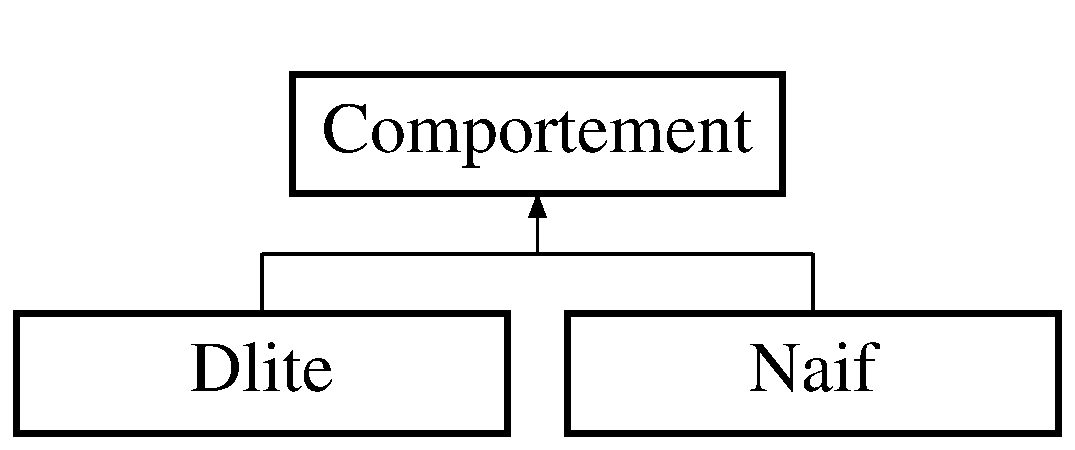
\includegraphics[height=2.000000cm]{class_comportement}
\end{center}
\end{figure}
\subsection*{Fonctions membres publiques}
\begin{DoxyCompactItemize}
\item 
\mbox{\hyperlink{class_comportement_a0c75007d7346cc14bb680eaa2981cb51}{Comportement}} ()
\item 
virtual \mbox{\hyperlink{class_comportement_acbe985635ed33cf141f380720c2e3f77}{$\sim$\+Comportement}} ()
\item 
virtual \mbox{\hyperlink{class_vecteur_r3}{Vecteur\+R3}} \mbox{\hyperlink{class_comportement_a38544976fc589cb8243c0c8071a692a6}{aller\+Point}} (const \mbox{\hyperlink{class_vecteur_r3}{Vecteur\+R3}} \&pos\+Actuelle, const \mbox{\hyperlink{class_vecteur_r3}{Vecteur\+R3}} \&destination, const std\+::vector$<$ \mbox{\hyperlink{class_capteur}{Capteur}} $>$ v\+Capteurs, const \mbox{\hyperlink{class_vecteur_r3}{Vecteur\+R3}} vitesse)=0
\end{DoxyCompactItemize}


\subsection{Description détaillée}
Interface donnant la fonction fondamentale de comportement de chaque \mbox{\hyperlink{class_drone}{Drone}}\+: le choix d\textquotesingle{}un nouveau vecteur accélération. \begin{DoxyAuthor}{Auteur}
Louis 
\end{DoxyAuthor}


\subsection{Documentation des constructeurs et destructeur}
\mbox{\Hypertarget{class_comportement_a0c75007d7346cc14bb680eaa2981cb51}\label{class_comportement_a0c75007d7346cc14bb680eaa2981cb51}} 
\index{Comportement@{Comportement}!Comportement@{Comportement}}
\index{Comportement@{Comportement}!Comportement@{Comportement}}
\subsubsection{\texorpdfstring{Comportement()}{Comportement()}}
{\footnotesize\ttfamily Comportement\+::\+Comportement (\begin{DoxyParamCaption}{ }\end{DoxyParamCaption})}

Constructeur vide. \mbox{\Hypertarget{class_comportement_acbe985635ed33cf141f380720c2e3f77}\label{class_comportement_acbe985635ed33cf141f380720c2e3f77}} 
\index{Comportement@{Comportement}!````~Comportement@{$\sim$\+Comportement}}
\index{````~Comportement@{$\sim$\+Comportement}!Comportement@{Comportement}}
\subsubsection{\texorpdfstring{$\sim$\+Comportement()}{~Comportement()}}
{\footnotesize\ttfamily Comportement\+::$\sim$\+Comportement (\begin{DoxyParamCaption}{ }\end{DoxyParamCaption})\hspace{0.3cm}{\ttfamily [virtual]}}

Destructeur vide. 

\subsection{Documentation des fonctions membres}
\mbox{\Hypertarget{class_comportement_a38544976fc589cb8243c0c8071a692a6}\label{class_comportement_a38544976fc589cb8243c0c8071a692a6}} 
\index{Comportement@{Comportement}!aller\+Point@{aller\+Point}}
\index{aller\+Point@{aller\+Point}!Comportement@{Comportement}}
\subsubsection{\texorpdfstring{aller\+Point()}{allerPoint()}}
{\footnotesize\ttfamily virtual \mbox{\hyperlink{class_vecteur_r3}{Vecteur\+R3}} Comportement\+::aller\+Point (\begin{DoxyParamCaption}\item[{const \mbox{\hyperlink{class_vecteur_r3}{Vecteur\+R3}} \&}]{pos\+Actuelle,  }\item[{const \mbox{\hyperlink{class_vecteur_r3}{Vecteur\+R3}} \&}]{destination,  }\item[{const std\+::vector$<$ \mbox{\hyperlink{class_capteur}{Capteur}} $>$}]{v\+Capteurs,  }\item[{const \mbox{\hyperlink{class_vecteur_r3}{Vecteur\+R3}}}]{vitesse }\end{DoxyParamCaption})\hspace{0.3cm}{\ttfamily [pure virtual]}}

Méthode fondamentale de \mbox{\hyperlink{class_comportement}{Comportement}} des Drones. A partir des positions du \mbox{\hyperlink{class_drone}{Drone}} et de son premier objectif, détermine (la méthode importe peu ici) le vecteur accélération pour la frame suivante. 
\begin{DoxyParams}{Paramètres}
{\em pos\+Actuelle} & la position du \mbox{\hyperlink{class_drone}{Drone}} au temps t. \\
\hline
{\em destination} & la position à atteindre. \\
\hline
{\em v\+Capteurs,le} & vecteur des Capteurs donnant l\textquotesingle{}information sensorielle du \mbox{\hyperlink{class_drone}{Drone}}. \\
\hline
\end{DoxyParams}
\begin{DoxyReturn}{Renvoie}
le vecteur accélération 
\end{DoxyReturn}


Implémenté dans \mbox{\hyperlink{class_naif_a67a1d4cfa924c6f1f2d8c1a9421ae120}{Naif}}.



La documentation de cette classe a été générée à partir des fichiers suivants \+:\begin{DoxyCompactItemize}
\item 
Comportement.\+h\item 
Comportement.\+cpp\end{DoxyCompactItemize}

\hypertarget{class_cubique}{}\section{Référence de la classe Cubique}
\label{class_cubique}\index{Cubique@{Cubique}}


{\ttfamily \#include $<$Cubique.\+h$>$}

Graphe d\textquotesingle{}héritage de Cubique\+:\begin{figure}[H]
\begin{center}
\leavevmode
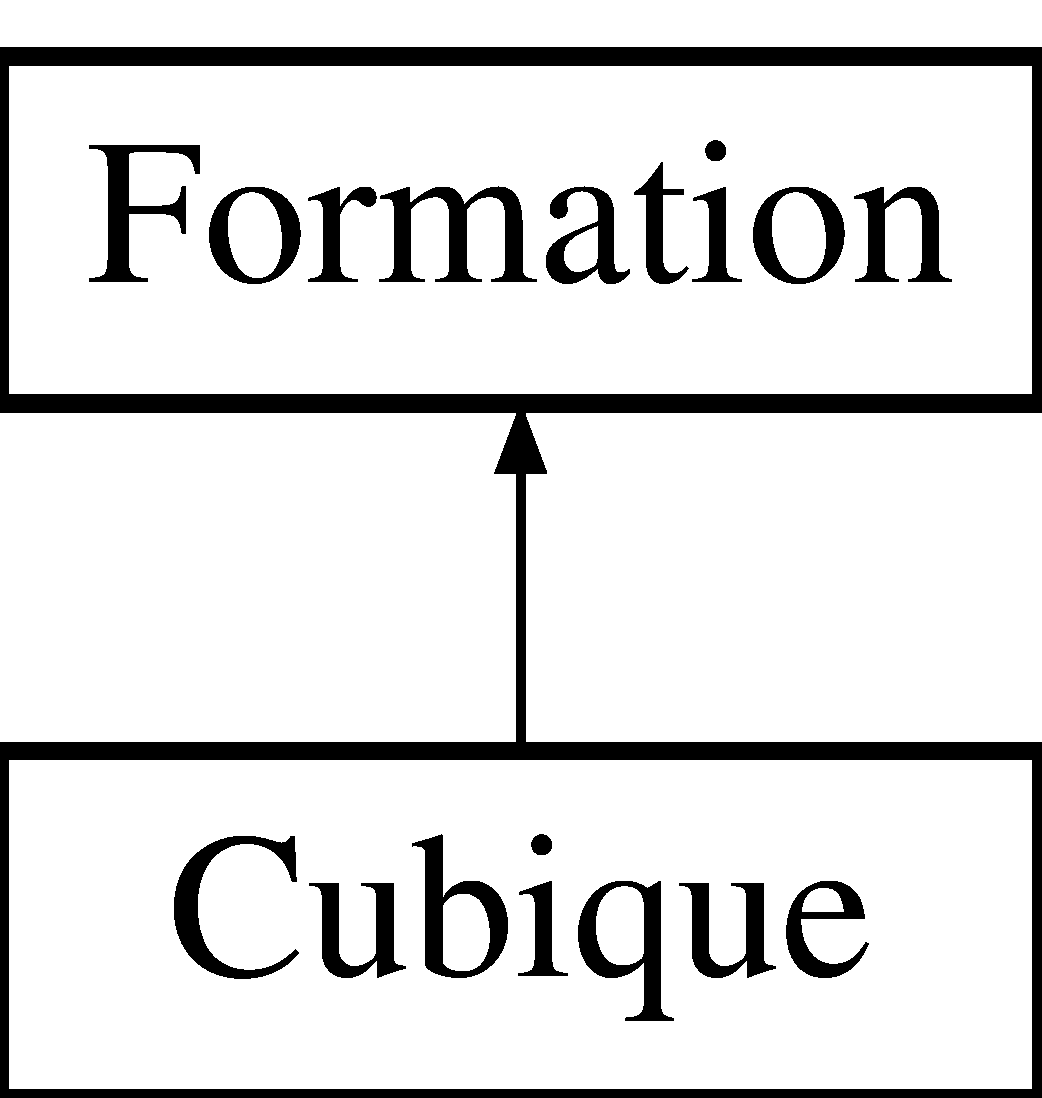
\includegraphics[height=2.000000cm]{class_cubique}
\end{center}
\end{figure}
\subsection*{Fonctions membres publiques}
\begin{DoxyCompactItemize}
\item 
\mbox{\hyperlink{class_cubique_ae437848fa7a382f250cf84d9b5c35154}{Cubique}} (\mbox{\hyperlink{class_vecteur_r3}{Vecteur\+R3}}, float, int)
\item 
virtual \mbox{\hyperlink{class_cubique_a5880f332af7c4f412b74ae9a6a71909a}{$\sim$\+Cubique}} ()
\item 
virtual vector$<$ \mbox{\hyperlink{class_vecteur_r3}{Vecteur\+R3}} $>$ \mbox{\hyperlink{class_cubique_ac7f56ed79d1732b2bf59e0456b3a2f6f}{generer\+Maillage}} ()
\end{DoxyCompactItemize}
\subsection*{Attributs protégés}
\begin{DoxyCompactItemize}
\item 
float \mbox{\hyperlink{class_cubique_a2d8ca11e6bf2f6b73aad6ca1f595990e}{longueur\+Cote}}
\item 
\mbox{\hyperlink{class_vecteur_r3}{Vecteur\+R3}} \mbox{\hyperlink{class_cubique_ab9d0ac86eeba76c72022bd84c401bb59}{origine}}
\end{DoxyCompactItemize}


\subsection{Description détaillée}
Classe fille de \mbox{\hyperlink{class_formation}{Formation}}, qui permet de dessiner un cube. \begin{DoxyAuthor}{Auteur}
Margot, Théau et Morgan 
\end{DoxyAuthor}
\begin{DoxyDate}{Date}
13/04/18 
\end{DoxyDate}


\subsection{Documentation des constructeurs et destructeur}
\mbox{\Hypertarget{class_cubique_ae437848fa7a382f250cf84d9b5c35154}\label{class_cubique_ae437848fa7a382f250cf84d9b5c35154}} 
\index{Cubique@{Cubique}!Cubique@{Cubique}}
\index{Cubique@{Cubique}!Cubique@{Cubique}}
\subsubsection{\texorpdfstring{Cubique()}{Cubique()}}
{\footnotesize\ttfamily Cubique\+::\+Cubique (\begin{DoxyParamCaption}\item[{\mbox{\hyperlink{class_vecteur_r3}{Vecteur\+R3}}}]{origine,  }\item[{float}]{longueur,  }\item[{int}]{nbre\+Drone }\end{DoxyParamCaption})}

Constructeur de la \mbox{\hyperlink{class_formation}{Formation}}. \mbox{\Hypertarget{class_cubique_a5880f332af7c4f412b74ae9a6a71909a}\label{class_cubique_a5880f332af7c4f412b74ae9a6a71909a}} 
\index{Cubique@{Cubique}!````~Cubique@{$\sim$\+Cubique}}
\index{````~Cubique@{$\sim$\+Cubique}!Cubique@{Cubique}}
\subsubsection{\texorpdfstring{$\sim$\+Cubique()}{~Cubique()}}
{\footnotesize\ttfamily Cubique\+::$\sim$\+Cubique (\begin{DoxyParamCaption}{ }\end{DoxyParamCaption})\hspace{0.3cm}{\ttfamily [virtual]}}

Destructeur usuel de la \mbox{\hyperlink{class_formation}{Formation}}. 

\subsection{Documentation des fonctions membres}
\mbox{\Hypertarget{class_cubique_ac7f56ed79d1732b2bf59e0456b3a2f6f}\label{class_cubique_ac7f56ed79d1732b2bf59e0456b3a2f6f}} 
\index{Cubique@{Cubique}!generer\+Maillage@{generer\+Maillage}}
\index{generer\+Maillage@{generer\+Maillage}!Cubique@{Cubique}}
\subsubsection{\texorpdfstring{generer\+Maillage()}{genererMaillage()}}
{\footnotesize\ttfamily vector$<$ \mbox{\hyperlink{class_vecteur_r3}{Vecteur\+R3}} $>$ Cubique\+::generer\+Maillage (\begin{DoxyParamCaption}{ }\end{DoxyParamCaption})\hspace{0.3cm}{\ttfamily [virtual]}}

Méthode héritée, calcule le maillage adapté à la formation cubique 

Implémente \mbox{\hyperlink{class_formation_ad1044228c0a1a4ee585ffe7f615c06ea}{Formation}}.



\subsection{Documentation des données membres}
\mbox{\Hypertarget{class_cubique_a2d8ca11e6bf2f6b73aad6ca1f595990e}\label{class_cubique_a2d8ca11e6bf2f6b73aad6ca1f595990e}} 
\index{Cubique@{Cubique}!longueur\+Cote@{longueur\+Cote}}
\index{longueur\+Cote@{longueur\+Cote}!Cubique@{Cubique}}
\subsubsection{\texorpdfstring{longueur\+Cote}{longueurCote}}
{\footnotesize\ttfamily float Cubique\+::longueur\+Cote\hspace{0.3cm}{\ttfamily [protected]}}

Longueur du côté du cube \mbox{\Hypertarget{class_cubique_ab9d0ac86eeba76c72022bd84c401bb59}\label{class_cubique_ab9d0ac86eeba76c72022bd84c401bb59}} 
\index{Cubique@{Cubique}!origine@{origine}}
\index{origine@{origine}!Cubique@{Cubique}}
\subsubsection{\texorpdfstring{origine}{origine}}
{\footnotesize\ttfamily \mbox{\hyperlink{class_vecteur_r3}{Vecteur\+R3}} Cubique\+::origine\hspace{0.3cm}{\ttfamily [protected]}}

Orgine du cube 

La documentation de cette classe a été générée à partir des fichiers suivants \+:\begin{DoxyCompactItemize}
\item 
Cubique.\+h\item 
Cubique.\+cpp\end{DoxyCompactItemize}

\hypertarget{class_dlite}{}\section{Référence de la classe Dlite}
\label{class_dlite}\index{Dlite@{Dlite}}


{\ttfamily \#include $<$Dlite.\+h$>$}

Graphe d\textquotesingle{}héritage de Dlite\+:\begin{figure}[H]
\begin{center}
\leavevmode
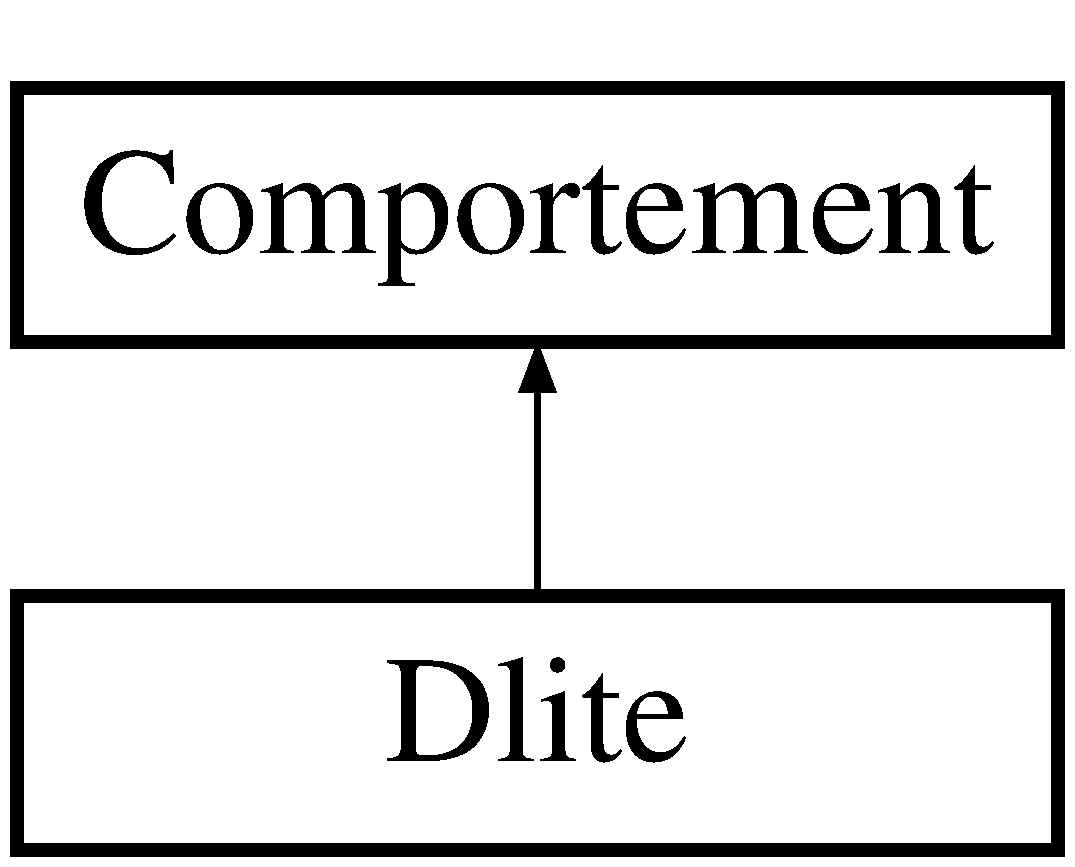
\includegraphics[height=2.000000cm]{class_dlite}
\end{center}
\end{figure}
\subsection*{Fonctions membres publiques}
\begin{DoxyCompactItemize}
\item 
\mbox{\hyperlink{class_dlite_a5f34443536a222e38f043d8370ca7b90}{Dlite}} ()
\item 
virtual \mbox{\hyperlink{class_dlite_ab98746140c7aa4ded45a47459b4c47d5}{$\sim$\+Dlite}} ()
\item 
\mbox{\hyperlink{class_vecteur_r3}{Vecteur\+R3}} \mbox{\hyperlink{class_dlite_a78c005fea65d3ae2429f74fd1d63c581}{aller\+Point}} (\mbox{\hyperlink{class_vecteur_r3}{Vecteur\+R3}} pos\+Actuelle, \mbox{\hyperlink{class_vecteur_r3}{Vecteur\+R3}} destination, std\+::vector$<$ \mbox{\hyperlink{class_capteur}{Capteur}} $>$ v\+Capteurs)
\end{DoxyCompactItemize}


\subsection{Description détaillée}
Type de \mbox{\hyperlink{class_comportement}{Comportement}}\+: algorithme \mbox{\hyperlink{class_dlite}{Dlite}}\+: amélioration dynamique de l\textquotesingle{}algorithme de pathfinding conventionnel A$\ast$. 

\subsection{Documentation des constructeurs et destructeur}
\mbox{\Hypertarget{class_dlite_a5f34443536a222e38f043d8370ca7b90}\label{class_dlite_a5f34443536a222e38f043d8370ca7b90}} 
\index{Dlite@{Dlite}!Dlite@{Dlite}}
\index{Dlite@{Dlite}!Dlite@{Dlite}}
\subsubsection{\texorpdfstring{Dlite()}{Dlite()}}
{\footnotesize\ttfamily Dlite\+::\+Dlite (\begin{DoxyParamCaption}{ }\end{DoxyParamCaption})}

Constructeur de l\textquotesingle{}algorithme. \mbox{\Hypertarget{class_dlite_ab98746140c7aa4ded45a47459b4c47d5}\label{class_dlite_ab98746140c7aa4ded45a47459b4c47d5}} 
\index{Dlite@{Dlite}!````~Dlite@{$\sim$\+Dlite}}
\index{````~Dlite@{$\sim$\+Dlite}!Dlite@{Dlite}}
\subsubsection{\texorpdfstring{$\sim$\+Dlite()}{~Dlite()}}
{\footnotesize\ttfamily Dlite\+::$\sim$\+Dlite (\begin{DoxyParamCaption}{ }\end{DoxyParamCaption})\hspace{0.3cm}{\ttfamily [virtual]}}

Destructeur de l\textquotesingle{}algorithme. 

\subsection{Documentation des fonctions membres}
\mbox{\Hypertarget{class_dlite_a78c005fea65d3ae2429f74fd1d63c581}\label{class_dlite_a78c005fea65d3ae2429f74fd1d63c581}} 
\index{Dlite@{Dlite}!aller\+Point@{aller\+Point}}
\index{aller\+Point@{aller\+Point}!Dlite@{Dlite}}
\subsubsection{\texorpdfstring{aller\+Point()}{allerPoint()}}
{\footnotesize\ttfamily \mbox{\hyperlink{class_vecteur_r3}{Vecteur\+R3}} Dlite\+::aller\+Point (\begin{DoxyParamCaption}\item[{\mbox{\hyperlink{class_vecteur_r3}{Vecteur\+R3}}}]{pos\+Actuelle,  }\item[{\mbox{\hyperlink{class_vecteur_r3}{Vecteur\+R3}}}]{destination,  }\item[{std\+::vector$<$ \mbox{\hyperlink{class_capteur}{Capteur}} $>$}]{v\+Capteurs }\end{DoxyParamCaption})}

Méthode fondamentale de \mbox{\hyperlink{class_comportement}{Comportement}} des Drones. A partir des positions du \mbox{\hyperlink{class_drone}{Drone}}, de son premier objectif et des capteurs, détermine le vecteur accélération pour la frame suivante. 
\begin{DoxyParams}{Paramètres}
{\em pos\+Actuelle} & la position du \mbox{\hyperlink{class_drone}{Drone}} au temps t. \\
\hline
{\em destination} & la position à atteindre. \\
\hline
{\em v\+Capteurs,le} & vecteur des Capteurs donnant l\textquotesingle{}information sensorielle du \mbox{\hyperlink{class_drone}{Drone}}. \\
\hline
\end{DoxyParams}
\begin{DoxyReturn}{Renvoie}
le vecteur accélération 
\end{DoxyReturn}


La documentation de cette classe a été générée à partir des fichiers suivants \+:\begin{DoxyCompactItemize}
\item 
Dlite.\+h\item 
Dlite.\+cpp\end{DoxyCompactItemize}

\hypertarget{class_drone}{}\section{Référence de la classe Drone}
\label{class_drone}\index{Drone@{Drone}}


{\ttfamily \#include $<$Drone.\+h$>$}

\subsection*{Fonctions membres publiques}
\begin{DoxyCompactItemize}
\item 
\mbox{\hyperlink{class_drone_a61e6934c19d51cecd69274b0c2f8f074}{Drone}} (const \mbox{\hyperlink{class_vecteur_r3}{Vecteur\+R3}})
\item 
\mbox{\hyperlink{class_drone_a1065b6a37230163bcd1b463c7a5121f7}{Drone}} (const float, const \mbox{\hyperlink{class_vecteur_r3}{Vecteur\+R3}}, const std\+::vector$<$ \mbox{\hyperlink{class_capteur}{Capteur}} $>$ \&)
\item 
\mbox{\hyperlink{class_drone_a11bd93fb5dccd88050ca2f89ab45617e}{Drone}} (const float rayon, \mbox{\hyperlink{class_vecteur_r3}{Vecteur\+R3}} pos, std\+::vector$<$ \mbox{\hyperlink{class_capteur}{Capteur}} $>$ v\+Cap, const \mbox{\hyperlink{class_vecteur_r3}{Vecteur\+R3}} \+\_\+gravite, \mbox{\hyperlink{class_vecteur_r3}{Vecteur\+R3}} vit=\mbox{\hyperlink{class_vecteur_r3}{Vecteur\+R3}}())
\item 
\mbox{\Hypertarget{class_drone_a0403556305197eda99c2f7305c03b7ac}\label{class_drone_a0403556305197eda99c2f7305c03b7ac}} 
\mbox{\hyperlink{class_drone}{Drone}} {\bfseries operator++} (int)
\item 
virtual \mbox{\hyperlink{class_drone_a667075abb1eb5c54be6418884a387d14}{$\sim$\+Drone}} ()
\item 
\mbox{\hyperlink{class_vecteur_r3}{Vecteur\+R3}} \mbox{\hyperlink{class_drone_ad8d5dda09c0e45c8d2c0f1f26a840f0e}{get\+Premier\+Objectif}} () const
\item 
std\+::queue$<$ \mbox{\hyperlink{class_vecteur_r3}{Vecteur\+R3}} $>$ \mbox{\hyperlink{class_drone_a11c5ec4c9211f217b2f0b11f46a1e627}{get\+V\+Objectifs}} () const
\item 
std\+::vector$<$ \mbox{\hyperlink{class_capteur}{Capteur}} $>$ \mbox{\hyperlink{class_drone_a0fb2eb8aa87f70b8f6d251f7b28feea4}{get\+V\+Capteurs}} () const
\item 
\mbox{\hyperlink{class_vecteur_r3}{Vecteur\+R3}} \mbox{\hyperlink{class_drone_a54d473991206bba12c44e5425779793e}{get\+Position}} () const
\item 
\mbox{\hyperlink{class_vecteur_r3}{Vecteur\+R3}} \mbox{\hyperlink{class_drone_a4b6a219813286c95545bccdf061a5f48}{get\+Vitesse}} () const
\item 
\mbox{\hyperlink{class_vecteur_r3}{Vecteur\+R3}} \mbox{\hyperlink{class_drone_a87ea8e6f37a123251b59ad936e51d4ad}{get\+Acceleration}} () const
\item 
void \mbox{\hyperlink{class_drone_a6a379b028a7c5b48bac16966fef5e1a4}{set\+Position}} (const \mbox{\hyperlink{class_vecteur_r3}{Vecteur\+R3}})
\item 
void \mbox{\hyperlink{class_drone_a63d698e315ebab5f36dd74447259828f}{set\+Vitesse}} (const \mbox{\hyperlink{class_vecteur_r3}{Vecteur\+R3}})
\item 
void \mbox{\hyperlink{class_drone_a75aaefd8ca47db757ad38a10482aa042}{set\+Acceleration}} (const \mbox{\hyperlink{class_vecteur_r3}{Vecteur\+R3}} \&)
\item 
float \mbox{\hyperlink{class_drone_a03a089698c78f9f4dedc51b5dc7099c3}{get\+Rayon}} () const
\item 
void \mbox{\hyperlink{class_drone_a0e15629285db6c6c9f1b21ce138bf6ec}{ne\+Fonctionne\+Plus}} ()
\item 
bool \mbox{\hyperlink{class_drone_a6df0c61c5aa61884d87365696f33affd}{est\+Fonctionnel}} () const
\item 
bool \mbox{\hyperlink{class_drone_a42c8991a71af54828612cba245b84063}{a\+Objectif}} () const
\item 
bool \mbox{\hyperlink{class_drone_a4e2e166a9a0c5732e789d08c6cda56d1}{atteint\+Objectif}} ()
\item 
bool \mbox{\hyperlink{class_drone_aaa8aa9eedb05b4c46bd92e88d5f14441}{porte\+Un\+Colis}} () const
\item 
void \mbox{\hyperlink{class_drone_aec517cb61a036852752219bad4e732c1}{ajouter\+Objectif}} (const \mbox{\hyperlink{class_vecteur_r3}{Vecteur\+R3}} \&obj)
\item 
void \mbox{\hyperlink{class_drone_ae7249a3f0c054e2c1beb6ea522774029}{livrer\+Colis}} (const \mbox{\hyperlink{class_vecteur_r3}{Vecteur\+R3}} \&retrait, const \mbox{\hyperlink{class_vecteur_r3}{Vecteur\+R3}} \&depot)
\end{DoxyCompactItemize}


\subsection{Description détaillée}
Agent du réseau qui a pour principale fonctionnalité de pouvoir se rendre d\textquotesingle{}un point à un autre, en suivant liste d\textquotesingle{}objectifs. Il se déplace en se donnant un vecteur accélération, qui donnera sa vitesse et position en temps t+1 via la classe \mbox{\hyperlink{class_environnement}{Environnement}}. \begin{DoxyAuthor}{Auteur}
Louis, Quentin 
\end{DoxyAuthor}


\subsection{Documentation des constructeurs et destructeur}
\mbox{\Hypertarget{class_drone_a61e6934c19d51cecd69274b0c2f8f074}\label{class_drone_a61e6934c19d51cecd69274b0c2f8f074}} 
\index{Drone@{Drone}!Drone@{Drone}}
\index{Drone@{Drone}!Drone@{Drone}}
\subsubsection{\texorpdfstring{Drone()}{Drone()}\hspace{0.1cm}{\footnotesize\ttfamily [1/3]}}
{\footnotesize\ttfamily Drone\+::\+Drone (\begin{DoxyParamCaption}\item[{const \mbox{\hyperlink{class_vecteur_r3}{Vecteur\+R3}}}]{pos }\end{DoxyParamCaption})}

Constructeur de \mbox{\hyperlink{class_drone}{Drone}} pour tests, avec position \mbox{\Hypertarget{class_drone_a1065b6a37230163bcd1b463c7a5121f7}\label{class_drone_a1065b6a37230163bcd1b463c7a5121f7}} 
\index{Drone@{Drone}!Drone@{Drone}}
\index{Drone@{Drone}!Drone@{Drone}}
\subsubsection{\texorpdfstring{Drone()}{Drone()}\hspace{0.1cm}{\footnotesize\ttfamily [2/3]}}
{\footnotesize\ttfamily Drone\+::\+Drone (\begin{DoxyParamCaption}\item[{const float}]{rayon\+Drone,  }\item[{const \mbox{\hyperlink{class_vecteur_r3}{Vecteur\+R3}}}]{pos,  }\item[{const std\+::vector$<$ \mbox{\hyperlink{class_capteur}{Capteur}} $>$ \&}]{v\+Cap }\end{DoxyParamCaption})}

Constructeur de test des Capteurs \mbox{\Hypertarget{class_drone_a11bd93fb5dccd88050ca2f89ab45617e}\label{class_drone_a11bd93fb5dccd88050ca2f89ab45617e}} 
\index{Drone@{Drone}!Drone@{Drone}}
\index{Drone@{Drone}!Drone@{Drone}}
\subsubsection{\texorpdfstring{Drone()}{Drone()}\hspace{0.1cm}{\footnotesize\ttfamily [3/3]}}
{\footnotesize\ttfamily Drone\+::\+Drone (\begin{DoxyParamCaption}\item[{const float}]{rayon,  }\item[{\mbox{\hyperlink{class_vecteur_r3}{Vecteur\+R3}}}]{pos,  }\item[{std\+::vector$<$ \mbox{\hyperlink{class_capteur}{Capteur}} $>$}]{v\+Cap,  }\item[{const \mbox{\hyperlink{class_vecteur_r3}{Vecteur\+R3}}}]{\+\_\+gravite,  }\item[{\mbox{\hyperlink{class_vecteur_r3}{Vecteur\+R3}}}]{vit = {\ttfamily \mbox{\hyperlink{class_vecteur_r3}{Vecteur\+R3}}()} }\end{DoxyParamCaption})}

Constructeur effectif de \mbox{\hyperlink{class_drone}{Drone}}. Prend une position et (éventuellement) vitesse initiales, un rayon et un vecteur de Capteurs. \mbox{\Hypertarget{class_drone_a667075abb1eb5c54be6418884a387d14}\label{class_drone_a667075abb1eb5c54be6418884a387d14}} 
\index{Drone@{Drone}!````~Drone@{$\sim$\+Drone}}
\index{````~Drone@{$\sim$\+Drone}!Drone@{Drone}}
\subsubsection{\texorpdfstring{$\sim$\+Drone()}{~Drone()}}
{\footnotesize\ttfamily Drone\+::$\sim$\+Drone (\begin{DoxyParamCaption}{ }\end{DoxyParamCaption})\hspace{0.3cm}{\ttfamily [virtual]}}

Destructeur de \mbox{\hyperlink{class_drone}{Drone}}. 

\subsection{Documentation des fonctions membres}
\mbox{\Hypertarget{class_drone_aec517cb61a036852752219bad4e732c1}\label{class_drone_aec517cb61a036852752219bad4e732c1}} 
\index{Drone@{Drone}!ajouter\+Objectif@{ajouter\+Objectif}}
\index{ajouter\+Objectif@{ajouter\+Objectif}!Drone@{Drone}}
\subsubsection{\texorpdfstring{ajouter\+Objectif()}{ajouterObjectif()}}
{\footnotesize\ttfamily void Drone\+::ajouter\+Objectif (\begin{DoxyParamCaption}\item[{const \mbox{\hyperlink{class_vecteur_r3}{Vecteur\+R3}} \&}]{obj }\end{DoxyParamCaption})}

Méthode qui ajoute une destination à la liste des objectifs. 
\begin{DoxyParams}{Paramètres}
{\em obj} & le point de R3 à ajouter à la liste d\textquotesingle{}objectifs. \\
\hline
\end{DoxyParams}
\mbox{\Hypertarget{class_drone_a42c8991a71af54828612cba245b84063}\label{class_drone_a42c8991a71af54828612cba245b84063}} 
\index{Drone@{Drone}!a\+Objectif@{a\+Objectif}}
\index{a\+Objectif@{a\+Objectif}!Drone@{Drone}}
\subsubsection{\texorpdfstring{a\+Objectif()}{aObjectif()}}
{\footnotesize\ttfamily bool Drone\+::a\+Objectif (\begin{DoxyParamCaption}{ }\end{DoxyParamCaption}) const}

Fonction qui indique si le drone a au moins un objectif (liste non nulle) \mbox{\Hypertarget{class_drone_a4e2e166a9a0c5732e789d08c6cda56d1}\label{class_drone_a4e2e166a9a0c5732e789d08c6cda56d1}} 
\index{Drone@{Drone}!atteint\+Objectif@{atteint\+Objectif}}
\index{atteint\+Objectif@{atteint\+Objectif}!Drone@{Drone}}
\subsubsection{\texorpdfstring{atteint\+Objectif()}{atteintObjectif()}}
{\footnotesize\ttfamily bool Drone\+::atteint\+Objectif (\begin{DoxyParamCaption}{ }\end{DoxyParamCaption})}

Teste si le drone a atteint son objectif. Le cas échéant, l\textquotesingle{}objectif est supprimé de la liste. \mbox{\Hypertarget{class_drone_a6df0c61c5aa61884d87365696f33affd}\label{class_drone_a6df0c61c5aa61884d87365696f33affd}} 
\index{Drone@{Drone}!est\+Fonctionnel@{est\+Fonctionnel}}
\index{est\+Fonctionnel@{est\+Fonctionnel}!Drone@{Drone}}
\subsubsection{\texorpdfstring{est\+Fonctionnel()}{estFonctionnel()}}
{\footnotesize\ttfamily bool Drone\+::est\+Fonctionnel (\begin{DoxyParamCaption}{ }\end{DoxyParamCaption}) const}

Getter sur l\textquotesingle{}état du drone \mbox{\Hypertarget{class_drone_a87ea8e6f37a123251b59ad936e51d4ad}\label{class_drone_a87ea8e6f37a123251b59ad936e51d4ad}} 
\index{Drone@{Drone}!get\+Acceleration@{get\+Acceleration}}
\index{get\+Acceleration@{get\+Acceleration}!Drone@{Drone}}
\subsubsection{\texorpdfstring{get\+Acceleration()}{getAcceleration()}}
{\footnotesize\ttfamily \mbox{\hyperlink{class_vecteur_r3}{Vecteur\+R3}} Drone\+::get\+Acceleration (\begin{DoxyParamCaption}{ }\end{DoxyParamCaption}) const}

Getter du vecteur acceleration \mbox{\Hypertarget{class_drone_a54d473991206bba12c44e5425779793e}\label{class_drone_a54d473991206bba12c44e5425779793e}} 
\index{Drone@{Drone}!get\+Position@{get\+Position}}
\index{get\+Position@{get\+Position}!Drone@{Drone}}
\subsubsection{\texorpdfstring{get\+Position()}{getPosition()}}
{\footnotesize\ttfamily \mbox{\hyperlink{class_vecteur_r3}{Vecteur\+R3}} Drone\+::get\+Position (\begin{DoxyParamCaption}{ }\end{DoxyParamCaption}) const}

Getter du vecteur position \mbox{\Hypertarget{class_drone_ad8d5dda09c0e45c8d2c0f1f26a840f0e}\label{class_drone_ad8d5dda09c0e45c8d2c0f1f26a840f0e}} 
\index{Drone@{Drone}!get\+Premier\+Objectif@{get\+Premier\+Objectif}}
\index{get\+Premier\+Objectif@{get\+Premier\+Objectif}!Drone@{Drone}}
\subsubsection{\texorpdfstring{get\+Premier\+Objectif()}{getPremierObjectif()}}
{\footnotesize\ttfamily \mbox{\hyperlink{class_vecteur_r3}{Vecteur\+R3}} Drone\+::get\+Premier\+Objectif (\begin{DoxyParamCaption}{ }\end{DoxyParamCaption}) const}

Getter du premier objectif du \mbox{\hyperlink{class_drone}{Drone}} \mbox{\Hypertarget{class_drone_a03a089698c78f9f4dedc51b5dc7099c3}\label{class_drone_a03a089698c78f9f4dedc51b5dc7099c3}} 
\index{Drone@{Drone}!get\+Rayon@{get\+Rayon}}
\index{get\+Rayon@{get\+Rayon}!Drone@{Drone}}
\subsubsection{\texorpdfstring{get\+Rayon()}{getRayon()}}
{\footnotesize\ttfamily float Drone\+::get\+Rayon (\begin{DoxyParamCaption}{ }\end{DoxyParamCaption}) const}

Getter du rayon du \mbox{\hyperlink{class_drone}{Drone}} \mbox{\Hypertarget{class_drone_a0fb2eb8aa87f70b8f6d251f7b28feea4}\label{class_drone_a0fb2eb8aa87f70b8f6d251f7b28feea4}} 
\index{Drone@{Drone}!get\+V\+Capteurs@{get\+V\+Capteurs}}
\index{get\+V\+Capteurs@{get\+V\+Capteurs}!Drone@{Drone}}
\subsubsection{\texorpdfstring{get\+V\+Capteurs()}{getVCapteurs()}}
{\footnotesize\ttfamily std\+::vector$<$ \mbox{\hyperlink{class_capteur}{Capteur}} $>$ Drone\+::get\+V\+Capteurs (\begin{DoxyParamCaption}{ }\end{DoxyParamCaption}) const}

Getter du vecteur de capteurs \mbox{\Hypertarget{class_drone_a4b6a219813286c95545bccdf061a5f48}\label{class_drone_a4b6a219813286c95545bccdf061a5f48}} 
\index{Drone@{Drone}!get\+Vitesse@{get\+Vitesse}}
\index{get\+Vitesse@{get\+Vitesse}!Drone@{Drone}}
\subsubsection{\texorpdfstring{get\+Vitesse()}{getVitesse()}}
{\footnotesize\ttfamily \mbox{\hyperlink{class_vecteur_r3}{Vecteur\+R3}} Drone\+::get\+Vitesse (\begin{DoxyParamCaption}{ }\end{DoxyParamCaption}) const}

Getter du vecteur vitesse \mbox{\Hypertarget{class_drone_a11c5ec4c9211f217b2f0b11f46a1e627}\label{class_drone_a11c5ec4c9211f217b2f0b11f46a1e627}} 
\index{Drone@{Drone}!get\+V\+Objectifs@{get\+V\+Objectifs}}
\index{get\+V\+Objectifs@{get\+V\+Objectifs}!Drone@{Drone}}
\subsubsection{\texorpdfstring{get\+V\+Objectifs()}{getVObjectifs()}}
{\footnotesize\ttfamily std\+::queue$<$ \mbox{\hyperlink{class_vecteur_r3}{Vecteur\+R3}} $>$ Drone\+::get\+V\+Objectifs (\begin{DoxyParamCaption}{ }\end{DoxyParamCaption}) const}

Getter des objectifs du \mbox{\hyperlink{class_drone}{Drone}} \mbox{\Hypertarget{class_drone_ae7249a3f0c054e2c1beb6ea522774029}\label{class_drone_ae7249a3f0c054e2c1beb6ea522774029}} 
\index{Drone@{Drone}!livrer\+Colis@{livrer\+Colis}}
\index{livrer\+Colis@{livrer\+Colis}!Drone@{Drone}}
\subsubsection{\texorpdfstring{livrer\+Colis()}{livrerColis()}}
{\footnotesize\ttfamily void Drone\+::livrer\+Colis (\begin{DoxyParamCaption}\item[{const \mbox{\hyperlink{class_vecteur_r3}{Vecteur\+R3}} \&}]{retrait,  }\item[{const \mbox{\hyperlink{class_vecteur_r3}{Vecteur\+R3}} \&}]{depot }\end{DoxyParamCaption})}

Ajoute à liste des objectifs le point de retrait et de dépôt du colis. 
\begin{DoxyParams}{Paramètres}
{\em retrait} & Le point auquel récupérer le colis. \\
\hline
{\em depot} & Le point auquel déposer le colis. \\
\hline
\end{DoxyParams}
\mbox{\Hypertarget{class_drone_a0e15629285db6c6c9f1b21ce138bf6ec}\label{class_drone_a0e15629285db6c6c9f1b21ce138bf6ec}} 
\index{Drone@{Drone}!ne\+Fonctionne\+Plus@{ne\+Fonctionne\+Plus}}
\index{ne\+Fonctionne\+Plus@{ne\+Fonctionne\+Plus}!Drone@{Drone}}
\subsubsection{\texorpdfstring{ne\+Fonctionne\+Plus()}{neFonctionnePlus()}}
{\footnotesize\ttfamily void Drone\+::ne\+Fonctionne\+Plus (\begin{DoxyParamCaption}{ }\end{DoxyParamCaption})}

affecte au bool \textquotesingle{}fonctionne\textquotesingle{} la valeur false. \mbox{\Hypertarget{class_drone_aaa8aa9eedb05b4c46bd92e88d5f14441}\label{class_drone_aaa8aa9eedb05b4c46bd92e88d5f14441}} 
\index{Drone@{Drone}!porte\+Un\+Colis@{porte\+Un\+Colis}}
\index{porte\+Un\+Colis@{porte\+Un\+Colis}!Drone@{Drone}}
\subsubsection{\texorpdfstring{porte\+Un\+Colis()}{porteUnColis()}}
{\footnotesize\ttfamily bool Drone\+::porte\+Un\+Colis (\begin{DoxyParamCaption}{ }\end{DoxyParamCaption}) const}

getter porte\+Colis \mbox{\Hypertarget{class_drone_a75aaefd8ca47db757ad38a10482aa042}\label{class_drone_a75aaefd8ca47db757ad38a10482aa042}} 
\index{Drone@{Drone}!set\+Acceleration@{set\+Acceleration}}
\index{set\+Acceleration@{set\+Acceleration}!Drone@{Drone}}
\subsubsection{\texorpdfstring{set\+Acceleration()}{setAcceleration()}}
{\footnotesize\ttfamily void Drone\+::set\+Acceleration (\begin{DoxyParamCaption}\item[{const \mbox{\hyperlink{class_vecteur_r3}{Vecteur\+R3}} \&}]{\+\_\+acc }\end{DoxyParamCaption})}

Setter du vecteur acceleration \mbox{\Hypertarget{class_drone_a6a379b028a7c5b48bac16966fef5e1a4}\label{class_drone_a6a379b028a7c5b48bac16966fef5e1a4}} 
\index{Drone@{Drone}!set\+Position@{set\+Position}}
\index{set\+Position@{set\+Position}!Drone@{Drone}}
\subsubsection{\texorpdfstring{set\+Position()}{setPosition()}}
{\footnotesize\ttfamily void Drone\+::set\+Position (\begin{DoxyParamCaption}\item[{const \mbox{\hyperlink{class_vecteur_r3}{Vecteur\+R3}}}]{nvll\+Pos }\end{DoxyParamCaption})}

Setter du vecteur position \mbox{\Hypertarget{class_drone_a63d698e315ebab5f36dd74447259828f}\label{class_drone_a63d698e315ebab5f36dd74447259828f}} 
\index{Drone@{Drone}!set\+Vitesse@{set\+Vitesse}}
\index{set\+Vitesse@{set\+Vitesse}!Drone@{Drone}}
\subsubsection{\texorpdfstring{set\+Vitesse()}{setVitesse()}}
{\footnotesize\ttfamily void Drone\+::set\+Vitesse (\begin{DoxyParamCaption}\item[{const \mbox{\hyperlink{class_vecteur_r3}{Vecteur\+R3}}}]{nvll\+Vit }\end{DoxyParamCaption})}

Setter du vecteur vitesse 

La documentation de cette classe a été générée à partir des fichiers suivants \+:\begin{DoxyCompactItemize}
\item 
Drone.\+h\item 
Drone.\+cpp\end{DoxyCompactItemize}

\hypertarget{class_environnement}{}\section{Référence de la classe Environnement}
\label{class_environnement}\index{Environnement@{Environnement}}


{\ttfamily \#include $<$Environnement.\+h$>$}

\subsection*{Fonctions membres publiques}
\begin{DoxyCompactItemize}
\item 
\mbox{\hyperlink{class_environnement_aebf8b1591072ad4585fec2db39942f60}{Environnement}} ()
\item 
\mbox{\hyperlink{class_environnement_a47869a858cb9d9ef3fdae28410646691}{Environnement}} (const float taille\+Cote)
\item 
\mbox{\Hypertarget{class_environnement_a465db1cf8ff840aa6d187a489225917b}\label{class_environnement_a465db1cf8ff840aa6d187a489225917b}} 
float {\bfseries get\+Cote} () const
\item 
\mbox{\Hypertarget{class_environnement_a9b81243bb194b219d0707480cc888144}\label{class_environnement_a9b81243bb194b219d0707480cc888144}} 
\mbox{\hyperlink{class_vecteur_r3}{Vecteur\+R3}} {\bfseries get\+Gravite} () const
\item 
\mbox{\Hypertarget{class_environnement_a4fced4e05ce0563a6e14f366b7ebe9ba}\label{class_environnement_a4fced4e05ce0563a6e14f366b7ebe9ba}} 
std\+::vector$<$ \mbox{\hyperlink{class_vecteur_r3}{Vecteur\+R3}} $>$ {\bfseries get\+V\+Retraits} () const
\item 
\mbox{\Hypertarget{class_environnement_ac9342b4f11be3856f129cb38590b43de}\label{class_environnement_ac9342b4f11be3856f129cb38590b43de}} 
std\+::vector$<$ \mbox{\hyperlink{class_vecteur_r3}{Vecteur\+R3}} $>$ {\bfseries get\+V\+Depots} () const
\item 
\mbox{\Hypertarget{class_environnement_aafb362bf7270314f8032e49f23ec3de2}\label{class_environnement_aafb362bf7270314f8032e49f23ec3de2}} 
\mbox{\hyperlink{class_vecteur_r3}{Vecteur\+R3}} {\bfseries get\+Origine\+Env} () const
\item 
\mbox{\Hypertarget{class_environnement_add48798bc7467e112020e8c0cf7f57ed}\label{class_environnement_add48798bc7467e112020e8c0cf7f57ed}} 
std\+::vector$<$ \mbox{\hyperlink{class_obstacle}{Obstacle}} $>$ {\bfseries get\+V\+Obstacles} () const
\item 
\mbox{\hyperlink{class_environnement}{Environnement}} \mbox{\hyperlink{class_environnement_aab744830dace48734c8fc02a594a4a30}{operator++}} (int)
\item 
void \mbox{\hyperlink{class_environnement_ae6251ccc61f336420464c300fdc87bb6}{ajouter\+Obstacle}} (const \mbox{\hyperlink{class_obstacle}{Obstacle}} \&)
\item 
void \mbox{\hyperlink{class_environnement_aab113d02197cc05b272ff66876cca4f1}{ajouter\+Colis}} (const \mbox{\hyperlink{class_vecteur_r3}{Vecteur\+R3}} \&, const \mbox{\hyperlink{class_vecteur_r3}{Vecteur\+R3}} \&)
\item 
void \mbox{\hyperlink{class_environnement_aa4a7722b750e7628f571c2915ac8d51f}{associer\+Essaim}} (\mbox{\hyperlink{class_essaim}{Essaim}} $\ast$)
\item 
std\+::vector$<$ \mbox{\hyperlink{class_drone}{Drone}} $\ast$ $>$ \mbox{\hyperlink{class_environnement_a22fcd53c6a16d7aac217000f04efb064}{get\+Essaim\+Drones}} () const
\end{DoxyCompactItemize}


\subsection{Description détaillée}
Classe contenant les éléments de l\textquotesingle{}environnement et leurs positions (i.\+e \mbox{\hyperlink{class_essaim}{Essaim}}, Obstacles, colis) Gère la détection de collision et le calcul de la position des drones. C\textquotesingle{}est le moteur physique du projet.

\begin{DoxyAuthor}{Auteurs}
Timothé, Simon 
\end{DoxyAuthor}


\subsection{Documentation des constructeurs et destructeur}
\mbox{\Hypertarget{class_environnement_aebf8b1591072ad4585fec2db39942f60}\label{class_environnement_aebf8b1591072ad4585fec2db39942f60}} 
\index{Environnement@{Environnement}!Environnement@{Environnement}}
\index{Environnement@{Environnement}!Environnement@{Environnement}}
\subsubsection{\texorpdfstring{Environnement()}{Environnement()}\hspace{0.1cm}{\footnotesize\ttfamily [1/2]}}
{\footnotesize\ttfamily Environnement\+::\+Environnement (\begin{DoxyParamCaption}{ }\end{DoxyParamCaption})}

Constructeur vide \mbox{\Hypertarget{class_environnement_a47869a858cb9d9ef3fdae28410646691}\label{class_environnement_a47869a858cb9d9ef3fdae28410646691}} 
\index{Environnement@{Environnement}!Environnement@{Environnement}}
\index{Environnement@{Environnement}!Environnement@{Environnement}}
\subsubsection{\texorpdfstring{Environnement()}{Environnement()}\hspace{0.1cm}{\footnotesize\ttfamily [2/2]}}
{\footnotesize\ttfamily Environnement\+::\+Environnement (\begin{DoxyParamCaption}\item[{const float}]{taille\+Cote }\end{DoxyParamCaption})}

Constructeur d\textquotesingle{}\mbox{\hyperlink{class_environnement}{Environnement}} avec la taille d\textquotesingle{}un côté. Le reste sera ajouté via les méthodes prévues à cet effet.

\begin{DoxyAuthor}{Auteurs}
Timothé, Simon, Théau 
\end{DoxyAuthor}


\subsection{Documentation des fonctions membres}
\mbox{\Hypertarget{class_environnement_aab113d02197cc05b272ff66876cca4f1}\label{class_environnement_aab113d02197cc05b272ff66876cca4f1}} 
\index{Environnement@{Environnement}!ajouter\+Colis@{ajouter\+Colis}}
\index{ajouter\+Colis@{ajouter\+Colis}!Environnement@{Environnement}}
\subsubsection{\texorpdfstring{ajouter\+Colis()}{ajouterColis()}}
{\footnotesize\ttfamily void Environnement\+::ajouter\+Colis (\begin{DoxyParamCaption}\item[{const \mbox{\hyperlink{class_vecteur_r3}{Vecteur\+R3}} \&}]{retrait,  }\item[{const \mbox{\hyperlink{class_vecteur_r3}{Vecteur\+R3}} \&}]{depot }\end{DoxyParamCaption})}

Ajoute un colis dans la liste à récupérer \mbox{\Hypertarget{class_environnement_ae6251ccc61f336420464c300fdc87bb6}\label{class_environnement_ae6251ccc61f336420464c300fdc87bb6}} 
\index{Environnement@{Environnement}!ajouter\+Obstacle@{ajouter\+Obstacle}}
\index{ajouter\+Obstacle@{ajouter\+Obstacle}!Environnement@{Environnement}}
\subsubsection{\texorpdfstring{ajouter\+Obstacle()}{ajouterObstacle()}}
{\footnotesize\ttfamily void Environnement\+::ajouter\+Obstacle (\begin{DoxyParamCaption}\item[{const \mbox{\hyperlink{class_obstacle}{Obstacle}} \&}]{obs }\end{DoxyParamCaption})}

Ajoute directement un objet \mbox{\hyperlink{class_obstacle}{Obstacle}} à la liste de l\textquotesingle{}\mbox{\hyperlink{class_environnement}{Environnement}} \mbox{\Hypertarget{class_environnement_aa4a7722b750e7628f571c2915ac8d51f}\label{class_environnement_aa4a7722b750e7628f571c2915ac8d51f}} 
\index{Environnement@{Environnement}!associer\+Essaim@{associer\+Essaim}}
\index{associer\+Essaim@{associer\+Essaim}!Environnement@{Environnement}}
\subsubsection{\texorpdfstring{associer\+Essaim()}{associerEssaim()}}
{\footnotesize\ttfamily void Environnement\+::associer\+Essaim (\begin{DoxyParamCaption}\item[{\mbox{\hyperlink{class_essaim}{Essaim}} $\ast$}]{e }\end{DoxyParamCaption})}

Donne sa valeur à l\textquotesingle{}attribut essaim une fois ce dernier créé (juste un set) \mbox{\Hypertarget{class_environnement_a22fcd53c6a16d7aac217000f04efb064}\label{class_environnement_a22fcd53c6a16d7aac217000f04efb064}} 
\index{Environnement@{Environnement}!get\+Essaim\+Drones@{get\+Essaim\+Drones}}
\index{get\+Essaim\+Drones@{get\+Essaim\+Drones}!Environnement@{Environnement}}
\subsubsection{\texorpdfstring{get\+Essaim\+Drones()}{getEssaimDrones()}}
{\footnotesize\ttfamily std\+::vector$<$ \mbox{\hyperlink{class_drone}{Drone}} $\ast$ $>$ Environnement\+::get\+Essaim\+Drones (\begin{DoxyParamCaption}{ }\end{DoxyParamCaption}) const}

Getter des Drones pour simplifier l\textquotesingle{}accès lors de l\textquotesingle{}affichage \mbox{\Hypertarget{class_environnement_aab744830dace48734c8fc02a594a4a30}\label{class_environnement_aab744830dace48734c8fc02a594a4a30}} 
\index{Environnement@{Environnement}!operator++@{operator++}}
\index{operator++@{operator++}!Environnement@{Environnement}}
\subsubsection{\texorpdfstring{operator++()}{operator++()}}
{\footnotesize\ttfamily \mbox{\hyperlink{class_environnement}{Environnement}} Environnement\+::operator++ (\begin{DoxyParamCaption}\item[{int}]{a }\end{DoxyParamCaption})}

Surchage de l\textquotesingle{}opérateur ++, afin de passer au temps+1 

La documentation de cette classe a été générée à partir des fichiers suivants \+:\begin{DoxyCompactItemize}
\item 
Environnement.\+h\item 
Environnement.\+cpp\end{DoxyCompactItemize}

\hypertarget{class_essaim}{}\section{Référence de la classe Essaim}
\label{class_essaim}\index{Essaim@{Essaim}}


{\ttfamily \#include $<$Essaim.\+h$>$}

\subsection*{Fonctions membres publiques}
\begin{DoxyCompactItemize}
\item 
\mbox{\hyperlink{class_essaim_a054ed8782a5d32914b820e635a0a1fdc}{Essaim}} ()
\item 
\mbox{\hyperlink{class_essaim_a1b2112a27d547ae2e19d75166b396886}{Essaim}} (\mbox{\hyperlink{class_environnement}{Environnement}} \&env, int nb\+Drones)
\item 
void \mbox{\hyperlink{class_essaim_a6e5a1427a3bdd7b7c7a29f07b54a5ae7}{retirer\+Colis}} (\mbox{\hyperlink{class_vecteur_r3}{Vecteur\+R3}} retrait, \mbox{\hyperlink{class_vecteur_r3}{Vecteur\+R3}} depot)
\item 
void \mbox{\hyperlink{class_essaim_acca17cbaea8479e9a6e1809e09bf913a}{formation}} (\mbox{\hyperlink{class_formation}{Formation}} \&F)
\item 
void \mbox{\hyperlink{class_essaim_a267e5067cbc6f33f3fa2b7e4e4a742a9}{ajouter\+Drone}} (\mbox{\hyperlink{class_drone}{Drone}} \&)
\item 
std\+::vector$<$ \mbox{\hyperlink{class_drone}{Drone}} $\ast$ $>$ \mbox{\hyperlink{class_essaim_a3910964b67c78a6897a723f9ed2972aa}{get\+V\+Drones}} () const
\end{DoxyCompactItemize}


\subsection{Description détaillée}
La classe \mbox{\hyperlink{class_essaim}{Essaim}} est celle qui contient l\textquotesingle{}ensemble des drones Elle a pour objectif de contrôler leurs objectifs (Attribution des colis aux drones, formations, ...)

\begin{DoxyAuthor}{Auteurs}
Timothé, Simon 
\end{DoxyAuthor}


\subsection{Documentation des constructeurs et destructeur}
\mbox{\Hypertarget{class_essaim_a054ed8782a5d32914b820e635a0a1fdc}\label{class_essaim_a054ed8782a5d32914b820e635a0a1fdc}} 
\index{Essaim@{Essaim}!Essaim@{Essaim}}
\index{Essaim@{Essaim}!Essaim@{Essaim}}
\subsubsection{\texorpdfstring{Essaim()}{Essaim()}\hspace{0.1cm}{\footnotesize\ttfamily [1/2]}}
{\footnotesize\ttfamily Essaim\+::\+Essaim (\begin{DoxyParamCaption}{ }\end{DoxyParamCaption})}

Constructeur vide \mbox{\Hypertarget{class_essaim_a1b2112a27d547ae2e19d75166b396886}\label{class_essaim_a1b2112a27d547ae2e19d75166b396886}} 
\index{Essaim@{Essaim}!Essaim@{Essaim}}
\index{Essaim@{Essaim}!Essaim@{Essaim}}
\subsubsection{\texorpdfstring{Essaim()}{Essaim()}\hspace{0.1cm}{\footnotesize\ttfamily [2/2]}}
{\footnotesize\ttfamily Essaim\+::\+Essaim (\begin{DoxyParamCaption}\item[{\mbox{\hyperlink{class_environnement}{Environnement}} \&}]{env,  }\item[{int}]{nb\+Drones }\end{DoxyParamCaption})}

Constructeur principal (utilisé dans le main de l\textquotesingle{}application) prenant l\textquotesingle{}\mbox{\hyperlink{class_environnement}{Environnement}} et le nombre de Drones 

\subsection{Documentation des fonctions membres}
\mbox{\Hypertarget{class_essaim_a267e5067cbc6f33f3fa2b7e4e4a742a9}\label{class_essaim_a267e5067cbc6f33f3fa2b7e4e4a742a9}} 
\index{Essaim@{Essaim}!ajouter\+Drone@{ajouter\+Drone}}
\index{ajouter\+Drone@{ajouter\+Drone}!Essaim@{Essaim}}
\subsubsection{\texorpdfstring{ajouter\+Drone()}{ajouterDrone()}}
{\footnotesize\ttfamily void Essaim\+::ajouter\+Drone (\begin{DoxyParamCaption}\item[{\mbox{\hyperlink{class_drone}{Drone}} \&}]{drone }\end{DoxyParamCaption})}

Ajoute un drone à l\textquotesingle{}essaim (dans le vector de drone) \mbox{\Hypertarget{class_essaim_acca17cbaea8479e9a6e1809e09bf913a}\label{class_essaim_acca17cbaea8479e9a6e1809e09bf913a}} 
\index{Essaim@{Essaim}!formation@{formation}}
\index{formation@{formation}!Essaim@{Essaim}}
\subsubsection{\texorpdfstring{formation()}{formation()}}
{\footnotesize\ttfamily void Essaim\+::formation (\begin{DoxyParamCaption}\item[{\mbox{\hyperlink{class_formation}{Formation}} \&}]{F }\end{DoxyParamCaption})}

Ordre aux drones de l\textquotesingle{}essaim de réaliser une formation \mbox{\Hypertarget{class_essaim_a3910964b67c78a6897a723f9ed2972aa}\label{class_essaim_a3910964b67c78a6897a723f9ed2972aa}} 
\index{Essaim@{Essaim}!get\+V\+Drones@{get\+V\+Drones}}
\index{get\+V\+Drones@{get\+V\+Drones}!Essaim@{Essaim}}
\subsubsection{\texorpdfstring{get\+V\+Drones()}{getVDrones()}}
{\footnotesize\ttfamily vector$<$ \mbox{\hyperlink{class_drone}{Drone}} $\ast$ $>$ Essaim\+::get\+V\+Drones (\begin{DoxyParamCaption}{ }\end{DoxyParamCaption}) const}

getter du vector de \mbox{\hyperlink{class_drone}{Drone}} \mbox{\Hypertarget{class_essaim_a6e5a1427a3bdd7b7c7a29f07b54a5ae7}\label{class_essaim_a6e5a1427a3bdd7b7c7a29f07b54a5ae7}} 
\index{Essaim@{Essaim}!retirer\+Colis@{retirer\+Colis}}
\index{retirer\+Colis@{retirer\+Colis}!Essaim@{Essaim}}
\subsubsection{\texorpdfstring{retirer\+Colis()}{retirerColis()}}
{\footnotesize\ttfamily void Essaim\+::retirer\+Colis (\begin{DoxyParamCaption}\item[{\mbox{\hyperlink{class_vecteur_r3}{Vecteur\+R3}}}]{retrait,  }\item[{\mbox{\hyperlink{class_vecteur_r3}{Vecteur\+R3}}}]{depot }\end{DoxyParamCaption})}

Ordre d\textquotesingle{}aller retirer un colis. Le drone qui doit aller le colis au point B est determiné dans le corps de la fonction et non passé en entrée 
\begin{DoxyParams}{Paramètres}
{\em retrait} & point de retrait du colis \\
\hline
{\em depot} & lieu où déposer le colis \\
\hline
\end{DoxyParams}


La documentation de cette classe a été générée à partir des fichiers suivants \+:\begin{DoxyCompactItemize}
\item 
Essaim.\+h\item 
Essaim.\+cpp\end{DoxyCompactItemize}

\hypertarget{class_formation}{}\section{Référence de la classe Formation}
\label{class_formation}\index{Formation@{Formation}}


{\ttfamily \#include $<$Formation.\+h$>$}

Graphe d\textquotesingle{}héritage de Formation\+:\begin{figure}[H]
\begin{center}
\leavevmode
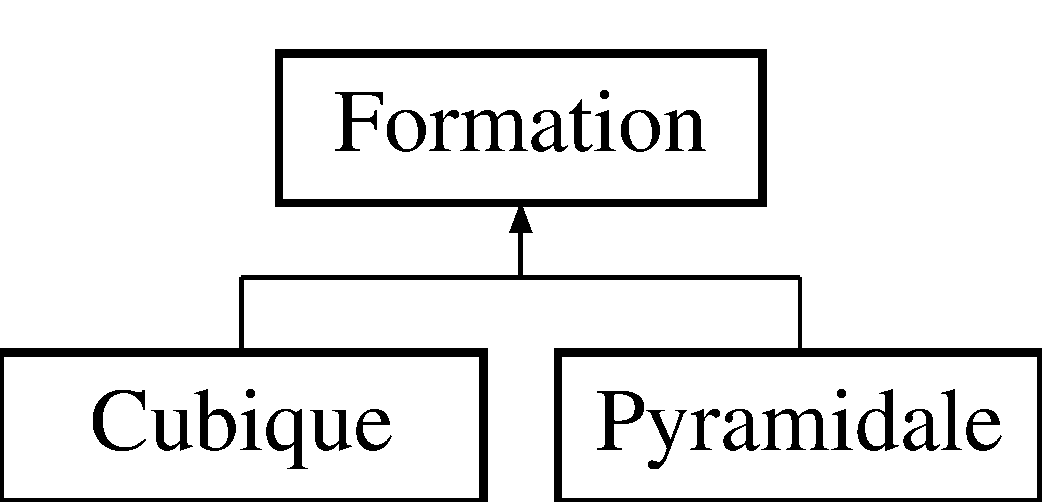
\includegraphics[height=2.000000cm]{class_formation}
\end{center}
\end{figure}
\subsection*{Fonctions membres publiques}
\begin{DoxyCompactItemize}
\item 
\mbox{\hyperlink{class_formation_a60c3058dd353550d89183ec529909cb6}{Formation}} ()
\item 
virtual \mbox{\hyperlink{class_formation_a5b4ffd37549ec211d85e52c916f35eb6}{$\sim$\+Formation}} ()
\item 
virtual vector$<$ \mbox{\hyperlink{class_vecteur_r3}{Vecteur\+R3}} $>$ \mbox{\hyperlink{class_formation_ad1044228c0a1a4ee585ffe7f615c06ea}{generer\+Maillage}} ()=0
\end{DoxyCompactItemize}
\subsection*{Attributs protégés}
\begin{DoxyCompactItemize}
\item 
float \mbox{\hyperlink{class_formation_a46ac97ac7c664d265c91a9ba3c718282}{altitude}}
\item 
int \mbox{\hyperlink{class_formation_a946670f42a19f84960990e9ffb781877}{nb\+Drones}}
\end{DoxyCompactItemize}


\subsection{Description détaillée}
Classe abstraite correspondant à une figure géométrique aérienne que peut réaliser une parte ou l\textquotesingle{}ensemble de l\textquotesingle{}essaim. \begin{DoxyAuthor}{Auteur}
Margot, Théau et Morgan 
\end{DoxyAuthor}
\begin{DoxyDate}{Date}
13/04/18 
\end{DoxyDate}


\subsection{Documentation des constructeurs et destructeur}
\mbox{\Hypertarget{class_formation_a60c3058dd353550d89183ec529909cb6}\label{class_formation_a60c3058dd353550d89183ec529909cb6}} 
\index{Formation@{Formation}!Formation@{Formation}}
\index{Formation@{Formation}!Formation@{Formation}}
\subsubsection{\texorpdfstring{Formation()}{Formation()}}
{\footnotesize\ttfamily Formation\+::\+Formation (\begin{DoxyParamCaption}{ }\end{DoxyParamCaption})}

Constructeur inutilisable (classe abstraite) \mbox{\Hypertarget{class_formation_a5b4ffd37549ec211d85e52c916f35eb6}\label{class_formation_a5b4ffd37549ec211d85e52c916f35eb6}} 
\index{Formation@{Formation}!````~Formation@{$\sim$\+Formation}}
\index{````~Formation@{$\sim$\+Formation}!Formation@{Formation}}
\subsubsection{\texorpdfstring{$\sim$\+Formation()}{~Formation()}}
{\footnotesize\ttfamily Formation\+::$\sim$\+Formation (\begin{DoxyParamCaption}{ }\end{DoxyParamCaption})\hspace{0.3cm}{\ttfamily [virtual]}}

Destructeur inutilisable (classe abstraite) 

\subsection{Documentation des fonctions membres}
\mbox{\Hypertarget{class_formation_ad1044228c0a1a4ee585ffe7f615c06ea}\label{class_formation_ad1044228c0a1a4ee585ffe7f615c06ea}} 
\index{Formation@{Formation}!generer\+Maillage@{generer\+Maillage}}
\index{generer\+Maillage@{generer\+Maillage}!Formation@{Formation}}
\subsubsection{\texorpdfstring{generer\+Maillage()}{genererMaillage()}}
{\footnotesize\ttfamily virtual vector$<$\mbox{\hyperlink{class_vecteur_r3}{Vecteur\+R3}}$>$ Formation\+::generer\+Maillage (\begin{DoxyParamCaption}{ }\end{DoxyParamCaption})\hspace{0.3cm}{\ttfamily [pure virtual]}}

Méthode permettant de générer le maillage à partir des points et des contraintes de taille de \mbox{\hyperlink{class_formation}{Formation}}. \begin{DoxyReturn}{Renvoie}
Retourne une nouvelle liste de vecteurs 
\end{DoxyReturn}


Implémenté dans \mbox{\hyperlink{class_cubique_ac7f56ed79d1732b2bf59e0456b3a2f6f}{Cubique}}.



\subsection{Documentation des données membres}
\mbox{\Hypertarget{class_formation_a46ac97ac7c664d265c91a9ba3c718282}\label{class_formation_a46ac97ac7c664d265c91a9ba3c718282}} 
\index{Formation@{Formation}!altitude@{altitude}}
\index{altitude@{altitude}!Formation@{Formation}}
\subsubsection{\texorpdfstring{altitude}{altitude}}
{\footnotesize\ttfamily float Formation\+::altitude\hspace{0.3cm}{\ttfamily [protected]}}

Altitude de la formation \mbox{\Hypertarget{class_formation_a946670f42a19f84960990e9ffb781877}\label{class_formation_a946670f42a19f84960990e9ffb781877}} 
\index{Formation@{Formation}!nb\+Drones@{nb\+Drones}}
\index{nb\+Drones@{nb\+Drones}!Formation@{Formation}}
\subsubsection{\texorpdfstring{nb\+Drones}{nbDrones}}
{\footnotesize\ttfamily int Formation\+::nb\+Drones\hspace{0.3cm}{\ttfamily [protected]}}

Le nombre de drones qui composent la formation 

La documentation de cette classe a été générée à partir des fichiers suivants \+:\begin{DoxyCompactItemize}
\item 
Formation.\+h\item 
Formation.\+cpp\end{DoxyCompactItemize}

\hypertarget{class_naif}{}\section{Référence de la classe Naif}
\label{class_naif}\index{Naif@{Naif}}


{\ttfamily \#include $<$Naif.\+h$>$}

Graphe d\textquotesingle{}héritage de Naif\+:\begin{figure}[H]
\begin{center}
\leavevmode
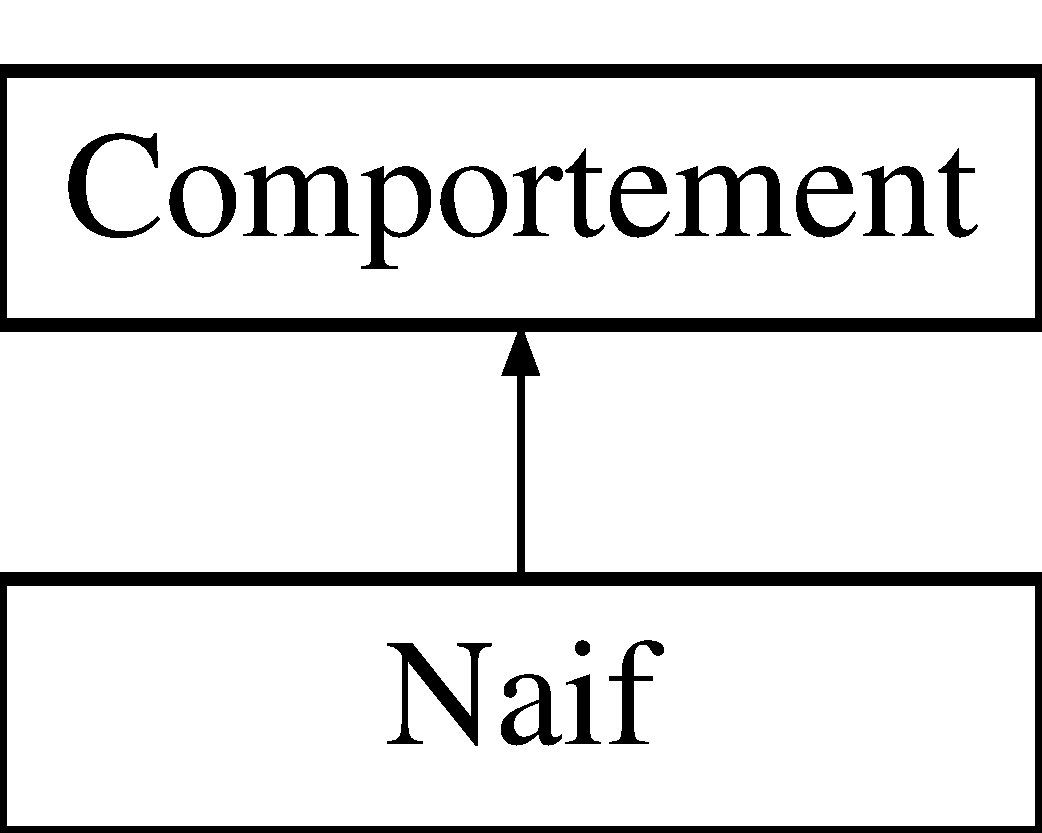
\includegraphics[height=2.000000cm]{class_naif}
\end{center}
\end{figure}
\subsection*{Fonctions membres publiques}
\begin{DoxyCompactItemize}
\item 
\mbox{\hyperlink{class_naif_acc816dcabca7caddbb282ec1bd232505}{Naif}} (const \mbox{\hyperlink{class_vecteur_r3}{Vecteur\+R3}}, const \mbox{\hyperlink{class_vecteur_r3}{Vecteur\+R3}})
\item 
virtual \mbox{\hyperlink{class_vecteur_r3}{Vecteur\+R3}} \mbox{\hyperlink{class_naif_a67a1d4cfa924c6f1f2d8c1a9421ae120}{aller\+Point}} (const \mbox{\hyperlink{class_vecteur_r3}{Vecteur\+R3}} \&pos\+Actuelle, const \mbox{\hyperlink{class_vecteur_r3}{Vecteur\+R3}} \&destination, const std\+::vector$<$ \mbox{\hyperlink{class_capteur}{Capteur}} $>$ v\+Capteurs, const \mbox{\hyperlink{class_vecteur_r3}{Vecteur\+R3}} vitesse) override
\item 
\mbox{\Hypertarget{class_naif_a71d7556cd1c9bc323820e052d34d2e2d}\label{class_naif_a71d7556cd1c9bc323820e052d34d2e2d}} 
bool {\bfseries atteint\+Final} (const \mbox{\hyperlink{class_vecteur_r3}{Vecteur\+R3}} \&pos\+Actuelle, const \mbox{\hyperlink{class_vecteur_r3}{Vecteur\+R3}} \&destination) const
\item 
\mbox{\Hypertarget{class_naif_aa5eaa77d98fe48768a8f6f031c287b8f}\label{class_naif_aa5eaa77d98fe48768a8f6f031c287b8f}} 
bool {\bfseries atteint} (const \mbox{\hyperlink{class_vecteur_r3}{Vecteur\+R3}} \&pos\+Actuelle, const \mbox{\hyperlink{class_vecteur_r3}{Vecteur\+R3}} \&destination, const float \&epsilon) const
\item 
\mbox{\Hypertarget{class_naif_a2bb16e2776f7e6cbb8cf75a4e78f6bc7}\label{class_naif_a2bb16e2776f7e6cbb8cf75a4e78f6bc7}} 
bool {\bfseries presence\+Obstacles} (const \mbox{\hyperlink{class_vecteur_r3}{Vecteur\+R3}} pos\+Actuelle, const \mbox{\hyperlink{class_vecteur_r3}{Vecteur\+R3}} destination, const std\+::vector$<$ \mbox{\hyperlink{class_capteur}{Capteur}} $>$ v\+Capteurs, const \mbox{\hyperlink{class_vecteur_r3}{Vecteur\+R3}} \&)
\end{DoxyCompactItemize}
\subsection*{Attributs publics}
\begin{DoxyCompactItemize}
\item 
\mbox{\hyperlink{class_vecteur_r3}{Vecteur\+R3}} \mbox{\hyperlink{class_naif_a0fde7dd2f98b4c8f163866ba7cd7d489}{depart}}
\item 
\mbox{\hyperlink{class_vecteur_r3}{Vecteur\+R3}} \mbox{\hyperlink{class_naif_a330eb7baf76efe3f36b7779669cccf64}{dest}}
\item 
\mbox{\hyperlink{class_vecteur_r3}{Vecteur\+R3}} \mbox{\hyperlink{class_naif_a11d7d76e77efcb9a2f47c4154bbfd55e}{v0}}
\end{DoxyCompactItemize}


\subsection{Description détaillée}
Classe héritant de \mbox{\hyperlink{class_comportement}{Comportement}}, c\textquotesingle{}est donc un algo possible de déplacement des drones. Il consiste à monter en altitude lorsque le drone rencontre un obstacle devant lui afin de passer au dessus.

\begin{DoxyAuthor}{Auteur}
Simon 
\end{DoxyAuthor}


\subsection{Documentation des constructeurs et destructeur}
\mbox{\Hypertarget{class_naif_acc816dcabca7caddbb282ec1bd232505}\label{class_naif_acc816dcabca7caddbb282ec1bd232505}} 
\index{Naif@{Naif}!Naif@{Naif}}
\index{Naif@{Naif}!Naif@{Naif}}
\subsubsection{\texorpdfstring{Naif()}{Naif()}}
{\footnotesize\ttfamily Naif\+::\+Naif (\begin{DoxyParamCaption}\item[{const \mbox{\hyperlink{class_vecteur_r3}{Vecteur\+R3}}}]{\+\_\+depart,  }\item[{const \mbox{\hyperlink{class_vecteur_r3}{Vecteur\+R3}}}]{\+\_\+v0 }\end{DoxyParamCaption})}

Initialise le point duquel le \mbox{\hyperlink{class_drone}{Drone}} part et sa vitesse 

\subsection{Documentation des fonctions membres}
\mbox{\Hypertarget{class_naif_a67a1d4cfa924c6f1f2d8c1a9421ae120}\label{class_naif_a67a1d4cfa924c6f1f2d8c1a9421ae120}} 
\index{Naif@{Naif}!aller\+Point@{aller\+Point}}
\index{aller\+Point@{aller\+Point}!Naif@{Naif}}
\subsubsection{\texorpdfstring{aller\+Point()}{allerPoint()}}
{\footnotesize\ttfamily \mbox{\hyperlink{class_vecteur_r3}{Vecteur\+R3}} Naif\+::aller\+Point (\begin{DoxyParamCaption}\item[{const \mbox{\hyperlink{class_vecteur_r3}{Vecteur\+R3}} \&}]{pos\+Actuelle,  }\item[{const \mbox{\hyperlink{class_vecteur_r3}{Vecteur\+R3}} \&}]{destination,  }\item[{const std\+::vector$<$ \mbox{\hyperlink{class_capteur}{Capteur}} $>$}]{v\+Capteurs,  }\item[{const \mbox{\hyperlink{class_vecteur_r3}{Vecteur\+R3}}}]{vitesse }\end{DoxyParamCaption})\hspace{0.3cm}{\ttfamily [override]}, {\ttfamily [virtual]}}

Méthode fondamentale de \mbox{\hyperlink{class_comportement}{Comportement}} des Drones. A partir des positions du \mbox{\hyperlink{class_drone}{Drone}}, de son premier objectif et des capteurs, d�termine le vecteur acc�l�ration pour la frame suivante. 
\begin{DoxyParams}{Paramètres}
{\em pos\+Actuelle} & la position du \mbox{\hyperlink{class_drone}{Drone}} au temps t. \\
\hline
{\em destination} & la position � atteindre. \\
\hline
{\em v\+Capteurs,le} & vecteur des Capteurs donnant l\textquotesingle{}information sensorielle du \mbox{\hyperlink{class_drone}{Drone}}. \\
\hline
\end{DoxyParams}
\begin{DoxyReturn}{Renvoie}
le vecteur acc�l�ration 
\end{DoxyReturn}


Implémente \mbox{\hyperlink{class_comportement_a38544976fc589cb8243c0c8071a692a6}{Comportement}}.



\subsection{Documentation des données membres}
\mbox{\Hypertarget{class_naif_a0fde7dd2f98b4c8f163866ba7cd7d489}\label{class_naif_a0fde7dd2f98b4c8f163866ba7cd7d489}} 
\index{Naif@{Naif}!depart@{depart}}
\index{depart@{depart}!Naif@{Naif}}
\subsubsection{\texorpdfstring{depart}{depart}}
{\footnotesize\ttfamily \mbox{\hyperlink{class_vecteur_r3}{Vecteur\+R3}} Naif\+::depart}

Position à laquelle le \mbox{\hyperlink{class_drone}{Drone}} a commencé à aller à l\textquotesingle{}objectif. Permet de réduire sa vitesse avant d\textquotesingle{}atteindre l\textquotesingle{}objectif. \mbox{\Hypertarget{class_naif_a330eb7baf76efe3f36b7779669cccf64}\label{class_naif_a330eb7baf76efe3f36b7779669cccf64}} 
\index{Naif@{Naif}!dest@{dest}}
\index{dest@{dest}!Naif@{Naif}}
\subsubsection{\texorpdfstring{dest}{dest}}
{\footnotesize\ttfamily \mbox{\hyperlink{class_vecteur_r3}{Vecteur\+R3}} Naif\+::dest}

Destination à atteindre. Permet de réinitialiser le depart en cas de changement d\textquotesingle{}objectif. \mbox{\Hypertarget{class_naif_a11d7d76e77efcb9a2f47c4154bbfd55e}\label{class_naif_a11d7d76e77efcb9a2f47c4154bbfd55e}} 
\index{Naif@{Naif}!v0@{v0}}
\index{v0@{v0}!Naif@{Naif}}
\subsubsection{\texorpdfstring{v0}{v0}}
{\footnotesize\ttfamily \mbox{\hyperlink{class_vecteur_r3}{Vecteur\+R3}} Naif\+::v0}

Vitesse à laquelle le drone est parti 

La documentation de cette classe a été générée à partir des fichiers suivants \+:\begin{DoxyCompactItemize}
\item 
Naif.\+h\item 
Naif.\+cpp\end{DoxyCompactItemize}

\hypertarget{class_obstacle}{}\section{Référence de la classe Obstacle}
\label{class_obstacle}\index{Obstacle@{Obstacle}}
\subsection*{Fonctions membres publiques}
\begin{DoxyCompactItemize}
\item 
\mbox{\hyperlink{class_obstacle_a72592db48f03233910c3c33145b96fd8}{Obstacle}} (\mbox{\hyperlink{class_vecteur_r3}{Vecteur\+R3}} init, float taillex, float tailley, float taillez)
\item 
vector$<$ \mbox{\hyperlink{class_vecteur_r3}{Vecteur\+R3}} $>$ \mbox{\hyperlink{class_obstacle_a5d69ba210a162084a37e246e3afc8574}{get\+V\+Sommets}} () const
\item 
vector$<$ \mbox{\hyperlink{class_vecteur_r3}{Vecteur\+R3}} $>$ \mbox{\hyperlink{class_obstacle_ac3d65b0cf5addfb7058e93d9fd36f8d2}{get\+Face\+Y\+Min}} () const
\item 
vector$<$ \mbox{\hyperlink{class_vecteur_r3}{Vecteur\+R3}} $>$ \mbox{\hyperlink{class_obstacle_abc88684297b935308cd23f0155df9fe9}{get\+Face\+Y\+Max}} () const
\item 
vector$<$ \mbox{\hyperlink{class_vecteur_r3}{Vecteur\+R3}} $>$ \mbox{\hyperlink{class_obstacle_ab0e0bd5dac1a93875b521536b65b148c}{get\+Face\+X\+Min}} () const
\item 
vector$<$ \mbox{\hyperlink{class_vecteur_r3}{Vecteur\+R3}} $>$ \mbox{\hyperlink{class_obstacle_a03ada1e0aaa5825666010b60a840bed4}{get\+Face\+X\+Max}} () const
\item 
vector$<$ \mbox{\hyperlink{class_vecteur_r3}{Vecteur\+R3}} $>$ \mbox{\hyperlink{class_obstacle_ae5d613bc2ff1f6c94e39db0855d63ade}{get\+Face\+Z\+Min}} () const
\item 
vector$<$ \mbox{\hyperlink{class_vecteur_r3}{Vecteur\+R3}} $>$ \mbox{\hyperlink{class_obstacle_a24887a162d5b7f8929c1bbae64bc70f5}{get\+Face\+Z\+Max}} () const
\item 
\mbox{\hyperlink{class_vecteur_r3}{Vecteur\+R3}} \mbox{\hyperlink{class_obstacle_a5f89117927ab1b5a3115f19ac21e0088}{get\+Centre}} () const
\item 
\mbox{\hyperlink{class_vecteur_r3}{Vecteur\+R3}} \mbox{\hyperlink{class_obstacle_a3520ca88bf9ea322647b1f3382dc0916}{get\+Init}} () const
\item 
float \mbox{\hyperlink{class_obstacle_a4cdb40f3bee6d9a9fad25ecfc831001f}{get\+TailleX}} () const
\item 
float \mbox{\hyperlink{class_obstacle_a14415e4953536b30e2ebf57112a92807}{get\+TailleY}} () const
\item 
float \mbox{\hyperlink{class_obstacle_ab2267f4612ffb80352494525040e8f91}{get\+TailleZ}} () const
\end{DoxyCompactItemize}


\subsection{Documentation des constructeurs et destructeur}
\mbox{\Hypertarget{class_obstacle_a72592db48f03233910c3c33145b96fd8}\label{class_obstacle_a72592db48f03233910c3c33145b96fd8}} 
\index{Obstacle@{Obstacle}!Obstacle@{Obstacle}}
\index{Obstacle@{Obstacle}!Obstacle@{Obstacle}}
\subsubsection{\texorpdfstring{Obstacle()}{Obstacle()}}
{\footnotesize\ttfamily Obstacle\+::\+Obstacle (\begin{DoxyParamCaption}\item[{\mbox{\hyperlink{class_vecteur_r3}{Vecteur\+R3}}}]{init,  }\item[{float}]{taillex,  }\item[{float}]{tailley,  }\item[{float}]{taillez }\end{DoxyParamCaption})}

Constructeur de pavé droit Ordre \+: base en horaire; haut en horaire (sens de rotation) 
\begin{DoxyParams}{Paramètres}
{\em init} & la position du coin aux coordonnées x,y,z minimales \\
\hline
\end{DoxyParams}


\subsection{Documentation des fonctions membres}
\mbox{\Hypertarget{class_obstacle_a5f89117927ab1b5a3115f19ac21e0088}\label{class_obstacle_a5f89117927ab1b5a3115f19ac21e0088}} 
\index{Obstacle@{Obstacle}!get\+Centre@{get\+Centre}}
\index{get\+Centre@{get\+Centre}!Obstacle@{Obstacle}}
\subsubsection{\texorpdfstring{get\+Centre()}{getCentre()}}
{\footnotesize\ttfamily \mbox{\hyperlink{class_vecteur_r3}{Vecteur\+R3}} Obstacle\+::get\+Centre (\begin{DoxyParamCaption}{ }\end{DoxyParamCaption}) const}

Getter centre \mbox{\Hypertarget{class_obstacle_a03ada1e0aaa5825666010b60a840bed4}\label{class_obstacle_a03ada1e0aaa5825666010b60a840bed4}} 
\index{Obstacle@{Obstacle}!get\+Face\+X\+Max@{get\+Face\+X\+Max}}
\index{get\+Face\+X\+Max@{get\+Face\+X\+Max}!Obstacle@{Obstacle}}
\subsubsection{\texorpdfstring{get\+Face\+X\+Max()}{getFaceXMax()}}
{\footnotesize\ttfamily vector$<$ \mbox{\hyperlink{class_vecteur_r3}{Vecteur\+R3}} $>$ Obstacle\+::get\+Face\+X\+Max (\begin{DoxyParamCaption}{ }\end{DoxyParamCaption}) const}

Getter face avant, X constant. (4 sommets) \mbox{\Hypertarget{class_obstacle_ab0e0bd5dac1a93875b521536b65b148c}\label{class_obstacle_ab0e0bd5dac1a93875b521536b65b148c}} 
\index{Obstacle@{Obstacle}!get\+Face\+X\+Min@{get\+Face\+X\+Min}}
\index{get\+Face\+X\+Min@{get\+Face\+X\+Min}!Obstacle@{Obstacle}}
\subsubsection{\texorpdfstring{get\+Face\+X\+Min()}{getFaceXMin()}}
{\footnotesize\ttfamily vector$<$ \mbox{\hyperlink{class_vecteur_r3}{Vecteur\+R3}} $>$ Obstacle\+::get\+Face\+X\+Min (\begin{DoxyParamCaption}{ }\end{DoxyParamCaption}) const}

Getter face arriere, X constant. (4 sommets) \mbox{\Hypertarget{class_obstacle_abc88684297b935308cd23f0155df9fe9}\label{class_obstacle_abc88684297b935308cd23f0155df9fe9}} 
\index{Obstacle@{Obstacle}!get\+Face\+Y\+Max@{get\+Face\+Y\+Max}}
\index{get\+Face\+Y\+Max@{get\+Face\+Y\+Max}!Obstacle@{Obstacle}}
\subsubsection{\texorpdfstring{get\+Face\+Y\+Max()}{getFaceYMax()}}
{\footnotesize\ttfamily vector$<$ \mbox{\hyperlink{class_vecteur_r3}{Vecteur\+R3}} $>$ Obstacle\+::get\+Face\+Y\+Max (\begin{DoxyParamCaption}{ }\end{DoxyParamCaption}) const}

Getter face droite, Y constant. (4 sommets) \mbox{\Hypertarget{class_obstacle_ac3d65b0cf5addfb7058e93d9fd36f8d2}\label{class_obstacle_ac3d65b0cf5addfb7058e93d9fd36f8d2}} 
\index{Obstacle@{Obstacle}!get\+Face\+Y\+Min@{get\+Face\+Y\+Min}}
\index{get\+Face\+Y\+Min@{get\+Face\+Y\+Min}!Obstacle@{Obstacle}}
\subsubsection{\texorpdfstring{get\+Face\+Y\+Min()}{getFaceYMin()}}
{\footnotesize\ttfamily vector$<$ \mbox{\hyperlink{class_vecteur_r3}{Vecteur\+R3}} $>$ Obstacle\+::get\+Face\+Y\+Min (\begin{DoxyParamCaption}{ }\end{DoxyParamCaption}) const}

Getter face gauche, Y constant. (4 sommets) \mbox{\Hypertarget{class_obstacle_a24887a162d5b7f8929c1bbae64bc70f5}\label{class_obstacle_a24887a162d5b7f8929c1bbae64bc70f5}} 
\index{Obstacle@{Obstacle}!get\+Face\+Z\+Max@{get\+Face\+Z\+Max}}
\index{get\+Face\+Z\+Max@{get\+Face\+Z\+Max}!Obstacle@{Obstacle}}
\subsubsection{\texorpdfstring{get\+Face\+Z\+Max()}{getFaceZMax()}}
{\footnotesize\ttfamily vector$<$ \mbox{\hyperlink{class_vecteur_r3}{Vecteur\+R3}} $>$ Obstacle\+::get\+Face\+Z\+Max (\begin{DoxyParamCaption}{ }\end{DoxyParamCaption}) const}

Getter face haute, Z constant. (4 sommets) \mbox{\Hypertarget{class_obstacle_ae5d613bc2ff1f6c94e39db0855d63ade}\label{class_obstacle_ae5d613bc2ff1f6c94e39db0855d63ade}} 
\index{Obstacle@{Obstacle}!get\+Face\+Z\+Min@{get\+Face\+Z\+Min}}
\index{get\+Face\+Z\+Min@{get\+Face\+Z\+Min}!Obstacle@{Obstacle}}
\subsubsection{\texorpdfstring{get\+Face\+Z\+Min()}{getFaceZMin()}}
{\footnotesize\ttfamily vector$<$ \mbox{\hyperlink{class_vecteur_r3}{Vecteur\+R3}} $>$ Obstacle\+::get\+Face\+Z\+Min (\begin{DoxyParamCaption}{ }\end{DoxyParamCaption}) const}

Getter face basse, Z constant. (4 sommets) \mbox{\Hypertarget{class_obstacle_a3520ca88bf9ea322647b1f3382dc0916}\label{class_obstacle_a3520ca88bf9ea322647b1f3382dc0916}} 
\index{Obstacle@{Obstacle}!get\+Init@{get\+Init}}
\index{get\+Init@{get\+Init}!Obstacle@{Obstacle}}
\subsubsection{\texorpdfstring{get\+Init()}{getInit()}}
{\footnotesize\ttfamily \mbox{\hyperlink{class_vecteur_r3}{Vecteur\+R3}} Obstacle\+::get\+Init (\begin{DoxyParamCaption}{ }\end{DoxyParamCaption}) const}

Getter point inital (coordonnées x,y,z minimales) \mbox{\Hypertarget{class_obstacle_a4cdb40f3bee6d9a9fad25ecfc831001f}\label{class_obstacle_a4cdb40f3bee6d9a9fad25ecfc831001f}} 
\index{Obstacle@{Obstacle}!get\+TailleX@{get\+TailleX}}
\index{get\+TailleX@{get\+TailleX}!Obstacle@{Obstacle}}
\subsubsection{\texorpdfstring{get\+Taille\+X()}{getTailleX()}}
{\footnotesize\ttfamily float Obstacle\+::get\+TailleX (\begin{DoxyParamCaption}{ }\end{DoxyParamCaption}) const}

Getter taille de cote en x \mbox{\Hypertarget{class_obstacle_a14415e4953536b30e2ebf57112a92807}\label{class_obstacle_a14415e4953536b30e2ebf57112a92807}} 
\index{Obstacle@{Obstacle}!get\+TailleY@{get\+TailleY}}
\index{get\+TailleY@{get\+TailleY}!Obstacle@{Obstacle}}
\subsubsection{\texorpdfstring{get\+Taille\+Y()}{getTailleY()}}
{\footnotesize\ttfamily float Obstacle\+::get\+TailleY (\begin{DoxyParamCaption}{ }\end{DoxyParamCaption}) const}

Getter taille de cote en y \mbox{\Hypertarget{class_obstacle_ab2267f4612ffb80352494525040e8f91}\label{class_obstacle_ab2267f4612ffb80352494525040e8f91}} 
\index{Obstacle@{Obstacle}!get\+TailleZ@{get\+TailleZ}}
\index{get\+TailleZ@{get\+TailleZ}!Obstacle@{Obstacle}}
\subsubsection{\texorpdfstring{get\+Taille\+Z()}{getTailleZ()}}
{\footnotesize\ttfamily float Obstacle\+::get\+TailleZ (\begin{DoxyParamCaption}{ }\end{DoxyParamCaption}) const}

Getter taille de cote en z \mbox{\Hypertarget{class_obstacle_a5d69ba210a162084a37e246e3afc8574}\label{class_obstacle_a5d69ba210a162084a37e246e3afc8574}} 
\index{Obstacle@{Obstacle}!get\+V\+Sommets@{get\+V\+Sommets}}
\index{get\+V\+Sommets@{get\+V\+Sommets}!Obstacle@{Obstacle}}
\subsubsection{\texorpdfstring{get\+V\+Sommets()}{getVSommets()}}
{\footnotesize\ttfamily vector$<$ \mbox{\hyperlink{class_vecteur_r3}{Vecteur\+R3}} $>$ Obstacle\+::get\+V\+Sommets (\begin{DoxyParamCaption}{ }\end{DoxyParamCaption}) const}

Renvoie le vector des sommets 

La documentation de cette classe a été générée à partir des fichiers suivants \+:\begin{DoxyCompactItemize}
\item 
Obstacle.\+h\item 
Obstacle.\+cpp\end{DoxyCompactItemize}

\hypertarget{class_pyramidale}{}\section{Référence de la classe Pyramidale}
\label{class_pyramidale}\index{Pyramidale@{Pyramidale}}


{\ttfamily \#include $<$Pyramidale.\+h$>$}

Graphe d\textquotesingle{}héritage de Pyramidale\+:\begin{figure}[H]
\begin{center}
\leavevmode
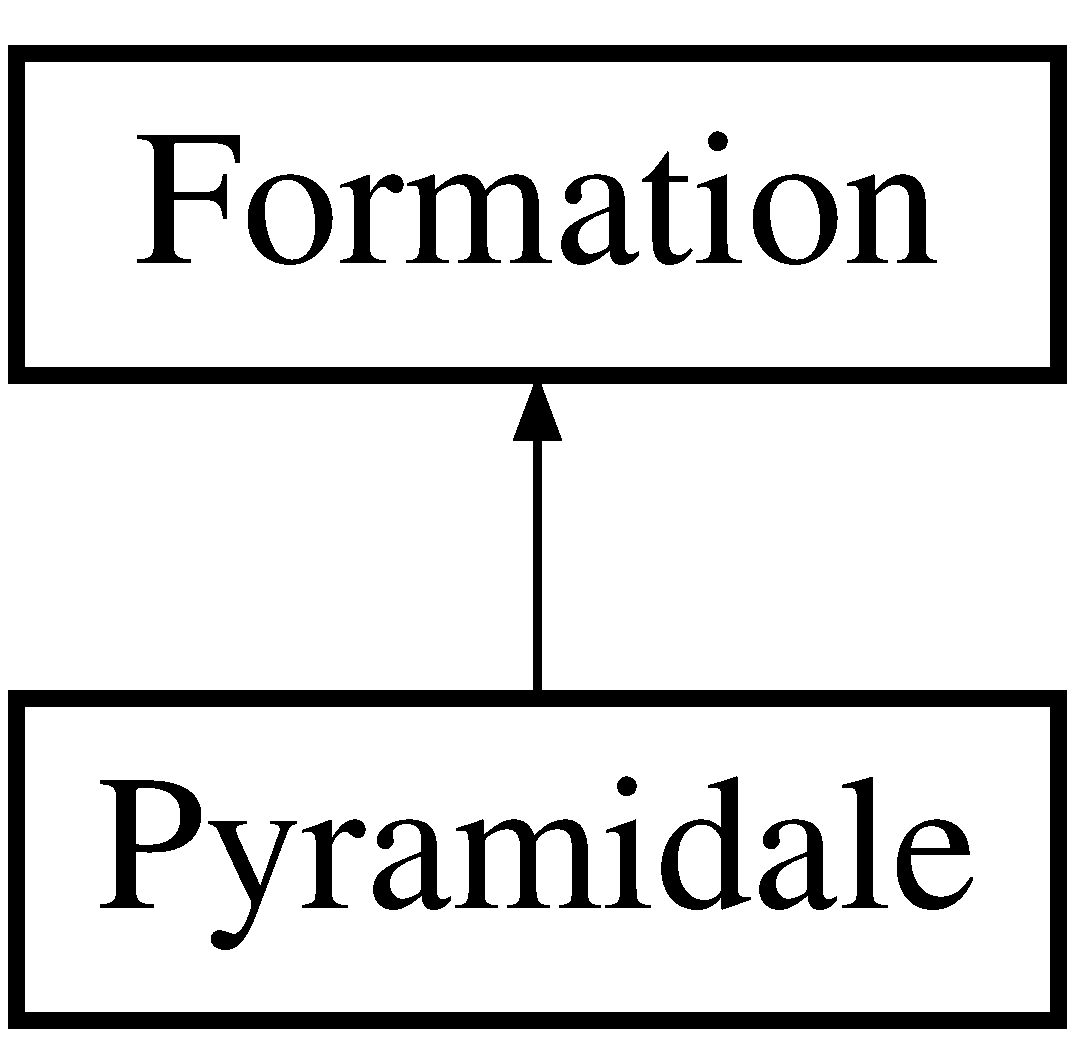
\includegraphics[height=2.000000cm]{class_pyramidale}
\end{center}
\end{figure}
\subsection*{Attributs protégés}
\begin{DoxyCompactItemize}
\item 
vector$<$ \mbox{\hyperlink{class_vecteur_r3}{Vecteur\+R3}} $>$ \mbox{\hyperlink{class_pyramidale_a3c8f1d8480417e91a65daa4f6d55c0ed}{v\+Points\+Base}}
\item 
\mbox{\hyperlink{class_vecteur_r3}{Vecteur\+R3}} \mbox{\hyperlink{class_pyramidale_a90a296c3487819ec38b5b9f7bbc13c8b}{sommet}}
\end{DoxyCompactItemize}
\subsection*{Membres hérités additionnels}


\subsection{Description détaillée}
Classe fille de \mbox{\hyperlink{class_formation}{Formation}}; dessine une pyramide. \begin{DoxyAuthor}{Auteur}
Margot, Théau et Morgan 
\end{DoxyAuthor}
\begin{DoxyDate}{Date}
13/04/18 
\end{DoxyDate}


\subsection{Documentation des données membres}
\mbox{\Hypertarget{class_pyramidale_a90a296c3487819ec38b5b9f7bbc13c8b}\label{class_pyramidale_a90a296c3487819ec38b5b9f7bbc13c8b}} 
\index{Pyramidale@{Pyramidale}!sommet@{sommet}}
\index{sommet@{sommet}!Pyramidale@{Pyramidale}}
\subsubsection{\texorpdfstring{sommet}{sommet}}
{\footnotesize\ttfamily \mbox{\hyperlink{class_vecteur_r3}{Vecteur\+R3}} Pyramidale\+::sommet\hspace{0.3cm}{\ttfamily [protected]}}

Point sommet de la pyramide \mbox{\Hypertarget{class_pyramidale_a3c8f1d8480417e91a65daa4f6d55c0ed}\label{class_pyramidale_a3c8f1d8480417e91a65daa4f6d55c0ed}} 
\index{Pyramidale@{Pyramidale}!v\+Points\+Base@{v\+Points\+Base}}
\index{v\+Points\+Base@{v\+Points\+Base}!Pyramidale@{Pyramidale}}
\subsubsection{\texorpdfstring{v\+Points\+Base}{vPointsBase}}
{\footnotesize\ttfamily vector$<$\mbox{\hyperlink{class_vecteur_r3}{Vecteur\+R3}}$>$ Pyramidale\+::v\+Points\+Base\hspace{0.3cm}{\ttfamily [protected]}}

Points formant la base de la pyramide 

La documentation de cette classe a été générée à partir des fichiers suivants \+:\begin{DoxyCompactItemize}
\item 
Pyramidale.\+h\item 
Pyramidale.\+cpp\end{DoxyCompactItemize}

\hypertarget{classtests_capteur}{}\section{Référence de la classe tests\+Capteur}
\label{classtests_capteur}\index{tests\+Capteur@{tests\+Capteur}}
Graphe d\textquotesingle{}héritage de tests\+Capteur\+:\begin{figure}[H]
\begin{center}
\leavevmode
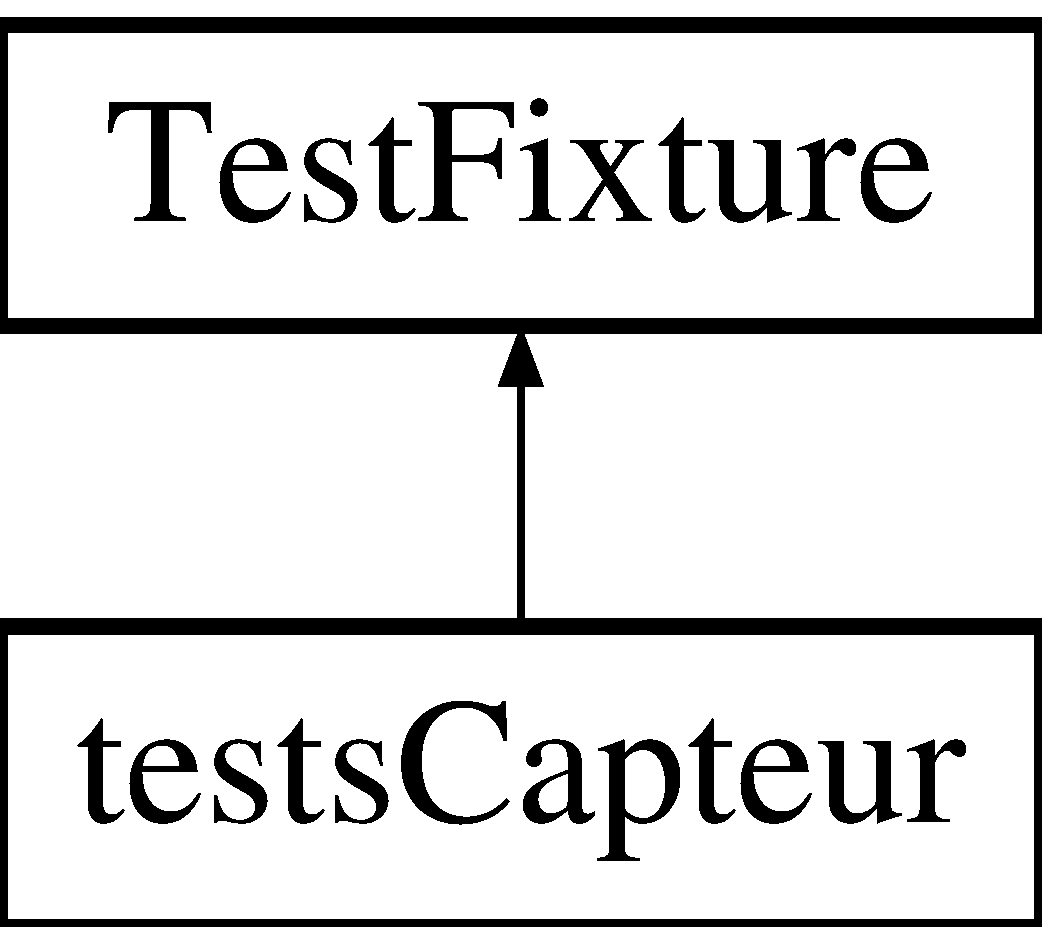
\includegraphics[height=2.000000cm]{classtests_capteur}
\end{center}
\end{figure}
\subsection*{Fonctions membres publiques}
\begin{DoxyCompactItemize}
\item 
\mbox{\Hypertarget{classtests_capteur_a6a2a2c663436fef1169276aa1fc9eb0c}\label{classtests_capteur_a6a2a2c663436fef1169276aa1fc9eb0c}} 
void {\bfseries set\+Up} (void)
\item 
\mbox{\Hypertarget{classtests_capteur_a009361891b05a8b2b8df71c28e593fe2}\label{classtests_capteur_a009361891b05a8b2b8df71c28e593fe2}} 
void {\bfseries tear\+Down} (void)
\end{DoxyCompactItemize}
\subsection*{Fonctions membres protégées}
\begin{DoxyCompactItemize}
\item 
void \mbox{\hyperlink{classtests_capteur_a7a72c1351f675987bbd5cbe70c91f33b}{test\+Update\+Distance\+Detectee}} (void)
\end{DoxyCompactItemize}


\subsection{Documentation des fonctions membres}
\mbox{\Hypertarget{classtests_capteur_a7a72c1351f675987bbd5cbe70c91f33b}\label{classtests_capteur_a7a72c1351f675987bbd5cbe70c91f33b}} 
\index{tests\+Capteur@{tests\+Capteur}!test\+Update\+Distance\+Detectee@{test\+Update\+Distance\+Detectee}}
\index{test\+Update\+Distance\+Detectee@{test\+Update\+Distance\+Detectee}!tests\+Capteur@{tests\+Capteur}}
\subsubsection{\texorpdfstring{test\+Update\+Distance\+Detectee()}{testUpdateDistanceDetectee()}}
{\footnotesize\ttfamily void tests\+Capteur\+::test\+Update\+Distance\+Detectee (\begin{DoxyParamCaption}\item[{void}]{ }\end{DoxyParamCaption})\hspace{0.3cm}{\ttfamily [protected]}}

Je lance la detection

Je vérifie que mon capteur detecte bien l\textquotesingle{}obstacle 

La documentation de cette classe a été générée à partir des fichiers suivants \+:\begin{DoxyCompactItemize}
\item 
tests\+Capteur.\+h\item 
tests\+Capteur.\+cpp\end{DoxyCompactItemize}

\hypertarget{classtests_drone}{}\section{Référence de la classe tests\+Drone}
\label{classtests_drone}\index{tests\+Drone@{tests\+Drone}}
Graphe d\textquotesingle{}héritage de tests\+Drone\+:\begin{figure}[H]
\begin{center}
\leavevmode
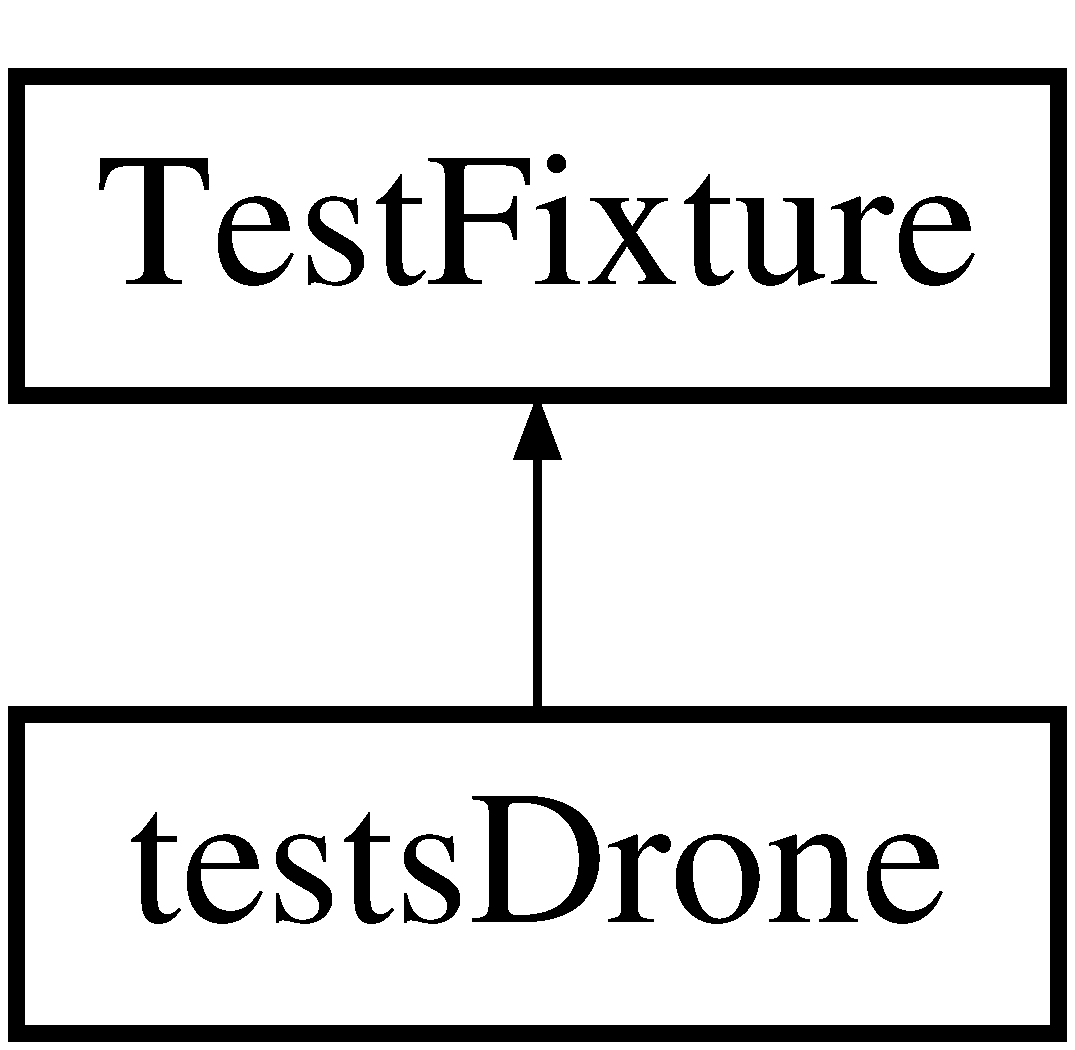
\includegraphics[height=2.000000cm]{classtests_drone}
\end{center}
\end{figure}
\subsection*{Fonctions membres publiques}
\begin{DoxyCompactItemize}
\item 
\mbox{\Hypertarget{classtests_drone_a82cd9f57ec465b41c6f2eec9e1bf1930}\label{classtests_drone_a82cd9f57ec465b41c6f2eec9e1bf1930}} 
void {\bfseries set\+Up} (void)
\item 
\mbox{\Hypertarget{classtests_drone_a89bb7ccbd1b705eb95c6efde0e4cc0cb}\label{classtests_drone_a89bb7ccbd1b705eb95c6efde0e4cc0cb}} 
void {\bfseries tear\+Down} (void)
\end{DoxyCompactItemize}
\subsection*{Fonctions membres protégées}
\begin{DoxyCompactItemize}
\item 
void \mbox{\hyperlink{classtests_drone_add1f7248206bee9d8e61ec4b2cd0731e}{test\+Ajouter\+Objectif}} ()
\item 
void \mbox{\hyperlink{classtests_drone_a6d3911d99922bf1a46f5209c66abe963}{test\+Livrer\+Colis}} ()
\item 
void \mbox{\hyperlink{classtests_drone_a3da2718fb45f6636f5f2d7c79030b418}{test\+Atteint\+Objectif}} ()
\item 
void \mbox{\hyperlink{classtests_drone_a7f3e884cbe3c28c276d7e9bae2b8bd53}{testplusplus}} ()
\end{DoxyCompactItemize}


\subsection{Documentation des fonctions membres}
\mbox{\Hypertarget{classtests_drone_add1f7248206bee9d8e61ec4b2cd0731e}\label{classtests_drone_add1f7248206bee9d8e61ec4b2cd0731e}} 
\index{tests\+Drone@{tests\+Drone}!test\+Ajouter\+Objectif@{test\+Ajouter\+Objectif}}
\index{test\+Ajouter\+Objectif@{test\+Ajouter\+Objectif}!tests\+Drone@{tests\+Drone}}
\subsubsection{\texorpdfstring{test\+Ajouter\+Objectif()}{testAjouterObjectif()}}
{\footnotesize\ttfamily void tests\+Drone\+::test\+Ajouter\+Objectif (\begin{DoxyParamCaption}{ }\end{DoxyParamCaption})\hspace{0.3cm}{\ttfamily [protected]}}

Teste l\textquotesingle{}ajout d\textquotesingle{}un objectif dans la liste des points à atteindre du \mbox{\hyperlink{class_drone}{Drone}}. A\+S\+S\+E\+RT si l\textquotesingle{}objectif a bien été ajouté; c\textquotesingle{}est-\/à-\/dire que la liste est plus grande d\textquotesingle{}un élément, qui est celui affiché. La vérification de la validité du point n\textquotesingle{}est pas du ressort du \mbox{\hyperlink{class_drone}{Drone}} (et donc de cette fonction). \mbox{\Hypertarget{classtests_drone_a3da2718fb45f6636f5f2d7c79030b418}\label{classtests_drone_a3da2718fb45f6636f5f2d7c79030b418}} 
\index{tests\+Drone@{tests\+Drone}!test\+Atteint\+Objectif@{test\+Atteint\+Objectif}}
\index{test\+Atteint\+Objectif@{test\+Atteint\+Objectif}!tests\+Drone@{tests\+Drone}}
\subsubsection{\texorpdfstring{test\+Atteint\+Objectif()}{testAtteintObjectif()}}
{\footnotesize\ttfamily void tests\+Drone\+::test\+Atteint\+Objectif (\begin{DoxyParamCaption}{ }\end{DoxyParamCaption})\hspace{0.3cm}{\ttfamily [protected]}}

Teste si l\textquotesingle{}objectif est bien considéré comme atteint et bien supprimé de la liste \mbox{\Hypertarget{classtests_drone_a6d3911d99922bf1a46f5209c66abe963}\label{classtests_drone_a6d3911d99922bf1a46f5209c66abe963}} 
\index{tests\+Drone@{tests\+Drone}!test\+Livrer\+Colis@{test\+Livrer\+Colis}}
\index{test\+Livrer\+Colis@{test\+Livrer\+Colis}!tests\+Drone@{tests\+Drone}}
\subsubsection{\texorpdfstring{test\+Livrer\+Colis()}{testLivrerColis()}}
{\footnotesize\ttfamily void tests\+Drone\+::test\+Livrer\+Colis (\begin{DoxyParamCaption}{ }\end{DoxyParamCaption})\hspace{0.3cm}{\ttfamily [protected]}}

Teste l\textquotesingle{}ordre de livraison de colis. Réalise globalement les mêmes tests que test\+Ajouter\+Objectif, sur deux points. \begin{DoxySeeAlso}{Voir également}
\mbox{\hyperlink{classtests_drone_add1f7248206bee9d8e61ec4b2cd0731e}{test\+Ajouter\+Objectif}} 
\end{DoxySeeAlso}
\mbox{\Hypertarget{classtests_drone_a7f3e884cbe3c28c276d7e9bae2b8bd53}\label{classtests_drone_a7f3e884cbe3c28c276d7e9bae2b8bd53}} 
\index{tests\+Drone@{tests\+Drone}!testplusplus@{testplusplus}}
\index{testplusplus@{testplusplus}!tests\+Drone@{tests\+Drone}}
\subsubsection{\texorpdfstring{testplusplus()}{testplusplus()}}
{\footnotesize\ttfamily void tests\+Drone\+::testplusplus (\begin{DoxyParamCaption}{ }\end{DoxyParamCaption})\hspace{0.3cm}{\ttfamily [protected]}}

Teste si la position est bien actualisé 

La documentation de cette classe a été générée à partir des fichiers suivants \+:\begin{DoxyCompactItemize}
\item 
tests\+Drone.\+h\item 
tests\+Drone.\+cpp\end{DoxyCompactItemize}

\hypertarget{classtests_environnement}{}\section{Référence de la classe tests\+Environnement}
\label{classtests_environnement}\index{tests\+Environnement@{tests\+Environnement}}
\subsection*{Fonctions membres publiques}
\begin{DoxyCompactItemize}
\item 
\mbox{\Hypertarget{classtests_environnement_abeba28862f0aec281c2fea8ea4a0b4ac}\label{classtests_environnement_abeba28862f0aec281c2fea8ea4a0b4ac}} 
void {\bfseries setup} (void)
\item 
\mbox{\Hypertarget{classtests_environnement_a328c941f6a50c7dba5eb22fbd2c952c0}\label{classtests_environnement_a328c941f6a50c7dba5eb22fbd2c952c0}} 
void {\bfseries tear\+Down} (void)
\end{DoxyCompactItemize}
\subsection*{Fonctions membres protégées}
\begin{DoxyCompactItemize}
\item 
\mbox{\Hypertarget{classtests_environnement_ae79caa635d1b58cc453b921797649056}\label{classtests_environnement_ae79caa635d1b58cc453b921797649056}} 
void {\bfseries testcalculer\+Pos} (void)
\item 
\mbox{\Hypertarget{classtests_environnement_a5d4b7e02dc219f13b240400476767b0d}\label{classtests_environnement_a5d4b7e02dc219f13b240400476767b0d}} 
void {\bfseries testcolision} (void)
\end{DoxyCompactItemize}


La documentation de cette classe a été générée à partir du fichier suivant \+:\begin{DoxyCompactItemize}
\item 
tests\+Environnement.\+h\end{DoxyCompactItemize}

\hypertarget{classtests_essaim}{}\section{Référence de la classe tests\+Essaim}
\label{classtests_essaim}\index{tests\+Essaim@{tests\+Essaim}}


{\ttfamily \#include $<$tests\+Essaim.\+h$>$}

Graphe d\textquotesingle{}héritage de tests\+Essaim\+:\begin{figure}[H]
\begin{center}
\leavevmode
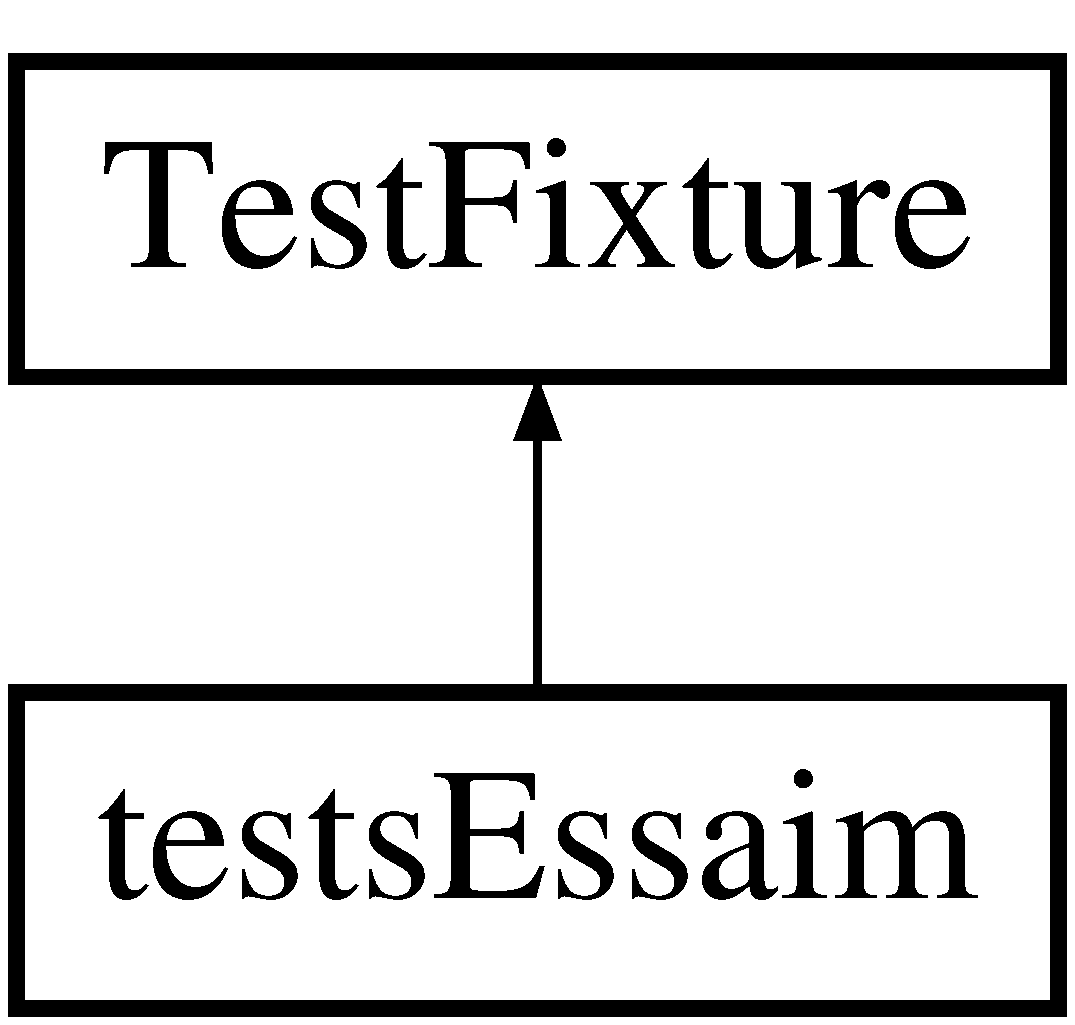
\includegraphics[height=2.000000cm]{classtests_essaim}
\end{center}
\end{figure}
\subsection*{Fonctions membres publiques}
\begin{DoxyCompactItemize}
\item 
\mbox{\Hypertarget{classtests_essaim_a11f3fd6586834e4fda0f7e2957e6f85d}\label{classtests_essaim_a11f3fd6586834e4fda0f7e2957e6f85d}} 
void {\bfseries set\+Up} (void)
\item 
\mbox{\Hypertarget{classtests_essaim_aeffed1c0f08751a477df994ba6e7dd48}\label{classtests_essaim_aeffed1c0f08751a477df994ba6e7dd48}} 
void {\bfseries tear\+Down} (void)
\end{DoxyCompactItemize}
\subsection*{Fonctions membres protégées}
\begin{DoxyCompactItemize}
\item 
\mbox{\Hypertarget{classtests_essaim_aecfe81de4a26fe35f16cfe73db6dd298}\label{classtests_essaim_aecfe81de4a26fe35f16cfe73db6dd298}} 
void {\bfseries test\+Ajouter\+Drone} ()
\item 
void \mbox{\hyperlink{classtests_essaim_ac6af8267d8e85120a6b1e5b66b247f5b}{test\+Retirer\+Colis}} ()
\item 
void \mbox{\hyperlink{classtests_essaim_a602aca58210132a947410123c130665e}{test\+Affectation\+Drone\+Pos}} ()
\end{DoxyCompactItemize}


\subsection{Description détaillée}
classe de test pour la classe \mbox{\hyperlink{class_essaim}{Essaim}} \begin{DoxyAuthor}{Auteur}
Simon 
\end{DoxyAuthor}


\subsection{Documentation des fonctions membres}
\mbox{\Hypertarget{classtests_essaim_a602aca58210132a947410123c130665e}\label{classtests_essaim_a602aca58210132a947410123c130665e}} 
\index{tests\+Essaim@{tests\+Essaim}!test\+Affectation\+Drone\+Pos@{test\+Affectation\+Drone\+Pos}}
\index{test\+Affectation\+Drone\+Pos@{test\+Affectation\+Drone\+Pos}!tests\+Essaim@{tests\+Essaim}}
\subsubsection{\texorpdfstring{test\+Affectation\+Drone\+Pos()}{testAffectationDronePos()}}
{\footnotesize\ttfamily void tests\+Essaim\+::test\+Affectation\+Drone\+Pos (\begin{DoxyParamCaption}{ }\end{DoxyParamCaption})\hspace{0.3cm}{\ttfamily [protected]}}

Appelle la fonction et vérifie si le bon \mbox{\hyperlink{class_drone}{Drone}} est bien dans la liste \mbox{\Hypertarget{classtests_essaim_ac6af8267d8e85120a6b1e5b66b247f5b}\label{classtests_essaim_ac6af8267d8e85120a6b1e5b66b247f5b}} 
\index{tests\+Essaim@{tests\+Essaim}!test\+Retirer\+Colis@{test\+Retirer\+Colis}}
\index{test\+Retirer\+Colis@{test\+Retirer\+Colis}!tests\+Essaim@{tests\+Essaim}}
\subsubsection{\texorpdfstring{test\+Retirer\+Colis()}{testRetirerColis()}}
{\footnotesize\ttfamily void tests\+Essaim\+::test\+Retirer\+Colis (\begin{DoxyParamCaption}{ }\end{DoxyParamCaption})\hspace{0.3cm}{\ttfamily [protected]}}

teste si la m�thode affecter\+Drone\+Pos affecte au drone le noeud du maillage le plus proche de sa position C\textquotesingle{}est une m�thode fastidieuse � tester. On va tester un exemple simple. Etant donn� 8 noeuds issus d\textquotesingle{}un maillage d\textquotesingle{}une formation cubique, on cr�� 8 drones l�g�rement d�cal� au 8 sommets. On v�rifie que chaque drone a comme objectif d\textquotesingle{}aller au sommet � cot� de lui. teste la m�thode retirer colis. On va faire apparaitre un colis a un endroit et on v�rifie que le drone le plus proche a bien re�u l\textquotesingle{}ordre de s\textquotesingle{}y rendre. Pour cela on regarde que les points de retrait et d�pose ont �t� ajout� � la liste des objectifs du drone le plus proche. 

La documentation de cette classe a été générée à partir des fichiers suivants \+:\begin{DoxyCompactItemize}
\item 
tests\+Essaim.\+h\item 
tests\+Essaim.\+cpp\end{DoxyCompactItemize}

\hypertarget{classtests_vecteur_r3}{}\section{Référence de la classe tests\+Vecteur\+R3}
\label{classtests_vecteur_r3}\index{tests\+Vecteur\+R3@{tests\+Vecteur\+R3}}
Graphe d\textquotesingle{}héritage de tests\+Vecteur\+R3\+:\begin{figure}[H]
\begin{center}
\leavevmode
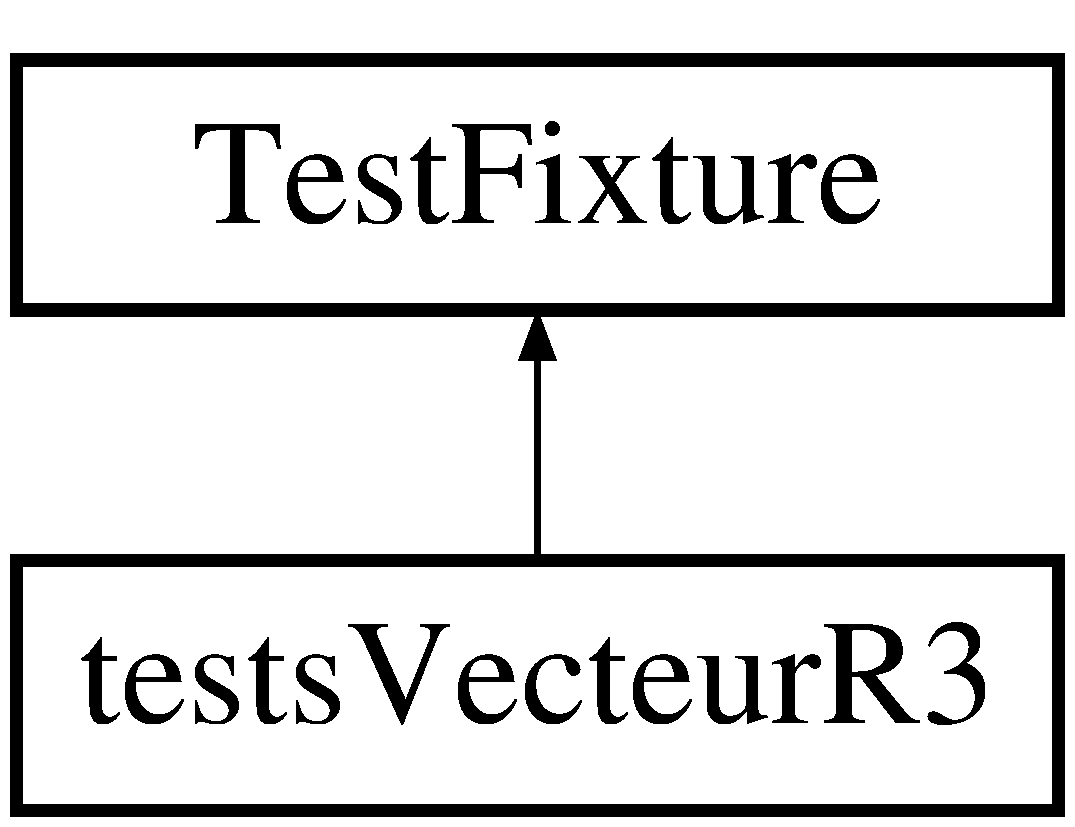
\includegraphics[height=2.000000cm]{classtests_vecteur_r3}
\end{center}
\end{figure}
\subsection*{Fonctions membres publiques}
\begin{DoxyCompactItemize}
\item 
\mbox{\Hypertarget{classtests_vecteur_r3_aab2c7d1043c9f9d55b55dfc273e0d932}\label{classtests_vecteur_r3_aab2c7d1043c9f9d55b55dfc273e0d932}} 
void {\bfseries set\+Up} (void)
\item 
\mbox{\Hypertarget{classtests_vecteur_r3_ac6f02917ca38304b46fe4660295bf3cc}\label{classtests_vecteur_r3_ac6f02917ca38304b46fe4660295bf3cc}} 
void {\bfseries tear\+Down} (void)
\end{DoxyCompactItemize}
\subsection*{Fonctions membres protégées}
\begin{DoxyCompactItemize}
\item 
\mbox{\Hypertarget{classtests_vecteur_r3_a66335d786c01247e7e0b819046f932b5}\label{classtests_vecteur_r3_a66335d786c01247e7e0b819046f932b5}} 
void {\bfseries test\+Egalite} (void)
\item 
\mbox{\Hypertarget{classtests_vecteur_r3_af8144f37bd755b4508a9cf3e55c6a336}\label{classtests_vecteur_r3_af8144f37bd755b4508a9cf3e55c6a336}} 
void {\bfseries test\+Addition} (void)
\item 
\mbox{\Hypertarget{classtests_vecteur_r3_a92455ad9ba84c67ef648ae6bbc58b39a}\label{classtests_vecteur_r3_a92455ad9ba84c67ef648ae6bbc58b39a}} 
void {\bfseries test\+Soustraction} (void)
\item 
\mbox{\Hypertarget{classtests_vecteur_r3_ab237e20bbd4d84b88650b6c3df4bcf08}\label{classtests_vecteur_r3_ab237e20bbd4d84b88650b6c3df4bcf08}} 
void {\bfseries test\+Multi} (void)
\item 
\mbox{\Hypertarget{classtests_vecteur_r3_ad55b4116890849c0eaceecf73ebe53a4}\label{classtests_vecteur_r3_ad55b4116890849c0eaceecf73ebe53a4}} 
void {\bfseries test\+Div} (void)
\item 
\mbox{\Hypertarget{classtests_vecteur_r3_a98889d942a2a3fd943618849e950700c}\label{classtests_vecteur_r3_a98889d942a2a3fd943618849e950700c}} 
void {\bfseries test\+Prod\+Scal} (void)
\item 
\mbox{\Hypertarget{classtests_vecteur_r3_ad587375a8995dfa2c2f4975b6ce6561f}\label{classtests_vecteur_r3_ad587375a8995dfa2c2f4975b6ce6561f}} 
void {\bfseries test\+Multiplication\+Scalaire} (void)
\item 
\mbox{\Hypertarget{classtests_vecteur_r3_a031400fd6b09207d81c0ee045bfb3fed}\label{classtests_vecteur_r3_a031400fd6b09207d81c0ee045bfb3fed}} 
void {\bfseries test\+Incrementation} (void)
\item 
\mbox{\Hypertarget{classtests_vecteur_r3_a1bdbc486011b693f5b9f52094ab5abe0}\label{classtests_vecteur_r3_a1bdbc486011b693f5b9f52094ab5abe0}} 
void {\bfseries test\+Norme22} (void)
\item 
\mbox{\Hypertarget{classtests_vecteur_r3_ad3141a4436113f0c43e0acbd661657b4}\label{classtests_vecteur_r3_ad3141a4436113f0c43e0acbd661657b4}} 
void {\bfseries testprod\+Vec} (void)
\item 
\mbox{\Hypertarget{classtests_vecteur_r3_af77c000809f77101f5e421a1741cf201}\label{classtests_vecteur_r3_af77c000809f77101f5e421a1741cf201}} 
void {\bfseries test\+Valeur\+Absolue} (void)
\item 
\mbox{\Hypertarget{classtests_vecteur_r3_a8e1b9c7fe6a23878f66fa6b82129f738}\label{classtests_vecteur_r3_a8e1b9c7fe6a23878f66fa6b82129f738}} 
void {\bfseries test\+Reflexion\+Plan\+Ortho} (void)
\end{DoxyCompactItemize}


La documentation de cette classe a été générée à partir des fichiers suivants \+:\begin{DoxyCompactItemize}
\item 
tests\+Vecteur\+R3.\+h\item 
tests\+Vecteur\+R3.\+cpp\end{DoxyCompactItemize}

\hypertarget{class_track_ball_camera}{}\section{Référence de la classe Track\+Ball\+Camera}
\label{class_track_ball_camera}\index{Track\+Ball\+Camera@{Track\+Ball\+Camera}}


{\ttfamily \#include $<$trackballcamera.\+h$>$}

\subsection*{Fonctions membres publiques}
\begin{DoxyCompactItemize}
\item 
\mbox{\Hypertarget{class_track_ball_camera_a7a700f13749637899fb8749e8d136598}\label{class_track_ball_camera_a7a700f13749637899fb8749e8d136598}} 
virtual void {\bfseries On\+Mouse\+Motion} (const S\+D\+L\+\_\+\+Mouse\+Motion\+Event \&event)
\item 
\mbox{\Hypertarget{class_track_ball_camera_a68e4695d4439a0f1a9dffdc474f9bcf2}\label{class_track_ball_camera_a68e4695d4439a0f1a9dffdc474f9bcf2}} 
virtual void {\bfseries On\+Mouse\+Button} (const S\+D\+L\+\_\+\+Mouse\+Button\+Event \&event)
\item 
\mbox{\Hypertarget{class_track_ball_camera_ac9d63bf5e2cc37176266d0f9002b6182}\label{class_track_ball_camera_ac9d63bf5e2cc37176266d0f9002b6182}} 
virtual void {\bfseries On\+Keyboard} (const S\+D\+L\+\_\+\+Keyboard\+Event \&event)
\item 
\mbox{\Hypertarget{class_track_ball_camera_ae7df52ed183dd63ec7ac6b6f4dd4f99d}\label{class_track_ball_camera_ae7df52ed183dd63ec7ac6b6f4dd4f99d}} 
virtual void {\bfseries look} ()
\item 
\mbox{\Hypertarget{class_track_ball_camera_a9942af262cd33039575f5c703304cc44}\label{class_track_ball_camera_a9942af262cd33039575f5c703304cc44}} 
virtual void {\bfseries set\+Motion\+Sensivity} (double sensivity)
\item 
\mbox{\Hypertarget{class_track_ball_camera_a55305b75b15ea49df24b89d591798661}\label{class_track_ball_camera_a55305b75b15ea49df24b89d591798661}} 
virtual void {\bfseries set\+Scroll\+Sensivity} (double sensivity)
\end{DoxyCompactItemize}
\subsection*{Attributs protégés}
\begin{DoxyCompactItemize}
\item 
\mbox{\Hypertarget{class_track_ball_camera_a097812817ed3ec665c76a38f71d8e133}\label{class_track_ball_camera_a097812817ed3ec665c76a38f71d8e133}} 
double {\bfseries \+\_\+motion\+Sensivity}
\item 
\mbox{\Hypertarget{class_track_ball_camera_ac24ec13cfb6134d7e064ba1052f08e23}\label{class_track_ball_camera_ac24ec13cfb6134d7e064ba1052f08e23}} 
double {\bfseries \+\_\+scroll\+Sensivity}
\item 
\mbox{\Hypertarget{class_track_ball_camera_a266fb5bce739065590ea94af85f6db96}\label{class_track_ball_camera_a266fb5bce739065590ea94af85f6db96}} 
bool {\bfseries \+\_\+hold}
\item 
\mbox{\Hypertarget{class_track_ball_camera_aeceb35b6b038fa4f756e5098b37ef9f4}\label{class_track_ball_camera_aeceb35b6b038fa4f756e5098b37ef9f4}} 
double {\bfseries \+\_\+distance}
\item 
\mbox{\Hypertarget{class_track_ball_camera_ad126b1c4d4e9e6bd8942015e7a19ebcc}\label{class_track_ball_camera_ad126b1c4d4e9e6bd8942015e7a19ebcc}} 
double {\bfseries \+\_\+angleY}
\item 
\mbox{\Hypertarget{class_track_ball_camera_a785783601aa752acffad8c227a486271}\label{class_track_ball_camera_a785783601aa752acffad8c227a486271}} 
double {\bfseries \+\_\+angleZ}
\item 
\mbox{\Hypertarget{class_track_ball_camera_ae9e9a83186de591c76ff43c7a1222d2b}\label{class_track_ball_camera_ae9e9a83186de591c76ff43c7a1222d2b}} 
S\+D\+L\+\_\+\+Cursor $\ast$ {\bfseries \+\_\+hand1}
\item 
\mbox{\Hypertarget{class_track_ball_camera_a3cf8251a5a65b3cf5b93ddbf811d165c}\label{class_track_ball_camera_a3cf8251a5a65b3cf5b93ddbf811d165c}} 
S\+D\+L\+\_\+\+Cursor $\ast$ {\bfseries \+\_\+hand2}
\end{DoxyCompactItemize}


\subsection{Description détaillée}
Class gestionnaire de tous les mouvements de la caméra; permet d\textquotesingle{}effectuer des rotations autour du centre à la souris. Récupéré d\textquotesingle{}Openclassrooms. \begin{DoxyAuthor}{Auteur}
Louis, Openclassrooms 
\end{DoxyAuthor}


La documentation de cette classe a été générée à partir des fichiers suivants \+:\begin{DoxyCompactItemize}
\item 
trackballcamera.\+h\item 
trackballcamera.\+cpp\end{DoxyCompactItemize}

\hypertarget{class_vecteur_r3}{}\section{Référence de la classe Vecteur\+R3}
\label{class_vecteur_r3}\index{Vecteur\+R3@{Vecteur\+R3}}


{\ttfamily \#include $<$Vecteur\+R3.\+h$>$}

\subsection*{Fonctions membres publiques}
\begin{DoxyCompactItemize}
\item 
\mbox{\hyperlink{class_vecteur_r3_a265cb675642abf1db0fbd99eed4590e7}{Vecteur\+R3}} ()
\item 
\mbox{\hyperlink{class_vecteur_r3_a86df8062a0522098bac7c2f18e97f2a3}{Vecteur\+R3}} (const float \&x, const float \&y, const float \&z)
\item 
virtual \mbox{\hyperlink{class_vecteur_r3_a75a59c365109680a59e84db71faf8eb9}{$\sim$\+Vecteur\+R3}} ()
\item 
\mbox{\Hypertarget{class_vecteur_r3_a715d8803e29c9c588f763ed2d7227f42}\label{class_vecteur_r3_a715d8803e29c9c588f763ed2d7227f42}} 
float {\bfseries getX} () const
\item 
\mbox{\Hypertarget{class_vecteur_r3_a5f019e331867afdb05cac782bb14e9e9}\label{class_vecteur_r3_a5f019e331867afdb05cac782bb14e9e9}} 
float {\bfseries getY} () const
\item 
\mbox{\Hypertarget{class_vecteur_r3_a144eb3201fcb8235f86ea56fbe60898f}\label{class_vecteur_r3_a144eb3201fcb8235f86ea56fbe60898f}} 
float {\bfseries getZ} () const
\item 
\mbox{\Hypertarget{class_vecteur_r3_a2d5f95e3b84ce304f46750e4d7d32505}\label{class_vecteur_r3_a2d5f95e3b84ce304f46750e4d7d32505}} 
void {\bfseries setX} (const float \&)
\item 
\mbox{\Hypertarget{class_vecteur_r3_a4ef6cac63a9a31d071dacea892129e47}\label{class_vecteur_r3_a4ef6cac63a9a31d071dacea892129e47}} 
void {\bfseries setY} (const float \&)
\item 
\mbox{\Hypertarget{class_vecteur_r3_a8266502ca7bdc70ec97672520f34b85f}\label{class_vecteur_r3_a8266502ca7bdc70ec97672520f34b85f}} 
void {\bfseries setZ} (const float \&)
\item 
float \mbox{\hyperlink{class_vecteur_r3_afb4fb3f4cd023a67cb74e906117ca30c}{operator\mbox{[}$\,$\mbox{]}}} (const int \&) const
\item 
\mbox{\Hypertarget{class_vecteur_r3_a0372c4411592d0a3adb4cf052e1b098d}\label{class_vecteur_r3_a0372c4411592d0a3adb4cf052e1b098d}} 
bool {\bfseries operator==} (const \mbox{\hyperlink{class_vecteur_r3}{Vecteur\+R3}} \&v\+Comp) const
\item 
bool \mbox{\hyperlink{class_vecteur_r3_a3e37c4a2e567844b4c32bede3f1b357e}{egal}} (const \mbox{\hyperlink{class_vecteur_r3}{Vecteur\+R3}} \&v\+Comp, const float \&epsilon=0) const
\item 
\mbox{\hyperlink{class_vecteur_r3}{Vecteur\+R3}} \mbox{\hyperlink{class_vecteur_r3_a00f29db8de9383f6627da7053c2c9af4}{operator+}} (const \mbox{\hyperlink{class_vecteur_r3}{Vecteur\+R3}} \&) const
\item 
\mbox{\hyperlink{class_vecteur_r3}{Vecteur\+R3}} \mbox{\hyperlink{class_vecteur_r3_a1a041eb37d796dcbb6e9a4d67df2e364}{operator-\/}} (const \mbox{\hyperlink{class_vecteur_r3}{Vecteur\+R3}} \&) const
\item 
\mbox{\hyperlink{class_vecteur_r3}{Vecteur\+R3}} \mbox{\hyperlink{class_vecteur_r3_adba111a3a9795f2cbeaa01efb99bb368}{div}} (const \mbox{\hyperlink{class_vecteur_r3}{Vecteur\+R3}} \&) const
\item 
\mbox{\hyperlink{class_vecteur_r3}{Vecteur\+R3}} \mbox{\hyperlink{class_vecteur_r3_ad03b38659a6e2454727487afb8842f0d}{multi}} (const \mbox{\hyperlink{class_vecteur_r3}{Vecteur\+R3}} \&) const
\item 
void \mbox{\hyperlink{class_vecteur_r3_ab001030cf179f0b78c4b57366132a87c}{operator=}} (const \mbox{\hyperlink{class_vecteur_r3}{Vecteur\+R3}} \&)
\item 
void \mbox{\hyperlink{class_vecteur_r3_ab50dc680b31f24957d39c60b63b71daf}{operator+=}} (const \mbox{\hyperlink{class_vecteur_r3}{Vecteur\+R3}} \&)
\item 
void \mbox{\hyperlink{class_vecteur_r3_a4cda50fa8f9233ed982d01b855cd6782}{operator-\/=}} (const \mbox{\hyperlink{class_vecteur_r3}{Vecteur\+R3}} \&)
\item 
float \mbox{\hyperlink{class_vecteur_r3_adba51a9c03c057ddafd76d4e62de3866}{operator$\ast$}} (const \mbox{\hyperlink{class_vecteur_r3}{Vecteur\+R3}} \&) const
\item 
\mbox{\hyperlink{class_vecteur_r3}{Vecteur\+R3}} \mbox{\hyperlink{class_vecteur_r3_a359b0ad02e7e539d32657d9722c620a6}{operator$\ast$}} (const float \&) const
\item 
float \mbox{\hyperlink{class_vecteur_r3_a014e36cfadce987c292edcf1db615cfd}{norme22}} () const
\item 
float \mbox{\hyperlink{class_vecteur_r3_a6c8bbc72999a06fd23e4213729f585b2}{norme2}} () const
\item 
\mbox{\hyperlink{class_vecteur_r3}{Vecteur\+R3}} \mbox{\hyperlink{class_vecteur_r3_a4fa29ea43737c79245a9ba049308d90b}{prod\+Vec}} (const \mbox{\hyperlink{class_vecteur_r3}{Vecteur\+R3}} \&) const
\item 
\mbox{\hyperlink{class_vecteur_r3}{Vecteur\+R3}} \mbox{\hyperlink{class_vecteur_r3_a9cef6d7525f81938e2a7e71aa73c442c}{valeur\+Absolue}} () const
\item 
\mbox{\hyperlink{class_vecteur_r3}{Vecteur\+R3}} \mbox{\hyperlink{class_vecteur_r3_a8191355529fdc2c4fa22cad27d6ad305}{reflexion\+Plan\+Ortho}} (const \mbox{\hyperlink{class_vecteur_r3}{Vecteur\+R3}} \&) const
\end{DoxyCompactItemize}
\subsection*{Amis}
\begin{DoxyCompactItemize}
\item 
std\+::ostream \& \mbox{\hyperlink{class_vecteur_r3_a1ef8b2a2f31c15f4f7765caad34796ca}{operator$<$$<$}} (std\+::ostream \&os, const \mbox{\hyperlink{class_vecteur_r3}{Vecteur\+R3}} \&)
\end{DoxyCompactItemize}


\subsection{Description détaillée}
Classe d\textquotesingle{}un vecteur dans R3, avec trois coordonnées et les opérations classiques des ensembles vectoriels. \begin{DoxyAuthor}{Auteurs}
\+: Margot, Morgan, Théau, Louis 
\end{DoxyAuthor}
\begin{DoxyVersion}{Version}
1.\+0 @13 avril 2018 
\end{DoxyVersion}


\subsection{Documentation des constructeurs et destructeur}
\mbox{\Hypertarget{class_vecteur_r3_a265cb675642abf1db0fbd99eed4590e7}\label{class_vecteur_r3_a265cb675642abf1db0fbd99eed4590e7}} 
\index{Vecteur\+R3@{Vecteur\+R3}!Vecteur\+R3@{Vecteur\+R3}}
\index{Vecteur\+R3@{Vecteur\+R3}!Vecteur\+R3@{Vecteur\+R3}}
\subsubsection{\texorpdfstring{Vecteur\+R3()}{VecteurR3()}\hspace{0.1cm}{\footnotesize\ttfamily [1/2]}}
{\footnotesize\ttfamily Vecteur\+R3\+::\+Vecteur\+R3 (\begin{DoxyParamCaption}{ }\end{DoxyParamCaption})}

Constructeur de \mbox{\hyperlink{class_vecteur_r3}{Vecteur\+R3}} initilisant les coordonnées à l\textquotesingle{}origine. \mbox{\Hypertarget{class_vecteur_r3_a86df8062a0522098bac7c2f18e97f2a3}\label{class_vecteur_r3_a86df8062a0522098bac7c2f18e97f2a3}} 
\index{Vecteur\+R3@{Vecteur\+R3}!Vecteur\+R3@{Vecteur\+R3}}
\index{Vecteur\+R3@{Vecteur\+R3}!Vecteur\+R3@{Vecteur\+R3}}
\subsubsection{\texorpdfstring{Vecteur\+R3()}{VecteurR3()}\hspace{0.1cm}{\footnotesize\ttfamily [2/2]}}
{\footnotesize\ttfamily Vecteur\+R3\+::\+Vecteur\+R3 (\begin{DoxyParamCaption}\item[{const float \&}]{x,  }\item[{const float \&}]{y,  }\item[{const float \&}]{z }\end{DoxyParamCaption})}

Constructeur de \mbox{\hyperlink{class_vecteur_r3}{Vecteur\+R3}} à partir de trois coordonnées données. \mbox{\Hypertarget{class_vecteur_r3_a75a59c365109680a59e84db71faf8eb9}\label{class_vecteur_r3_a75a59c365109680a59e84db71faf8eb9}} 
\index{Vecteur\+R3@{Vecteur\+R3}!````~Vecteur\+R3@{$\sim$\+Vecteur\+R3}}
\index{````~Vecteur\+R3@{$\sim$\+Vecteur\+R3}!Vecteur\+R3@{Vecteur\+R3}}
\subsubsection{\texorpdfstring{$\sim$\+Vecteur\+R3()}{~VecteurR3()}}
{\footnotesize\ttfamily Vecteur\+R3\+::$\sim$\+Vecteur\+R3 (\begin{DoxyParamCaption}{ }\end{DoxyParamCaption})\hspace{0.3cm}{\ttfamily [virtual]}}

Destructeur d\textquotesingle{}un \mbox{\hyperlink{class_vecteur_r3}{Vecteur\+R3}}. 

\subsection{Documentation des fonctions membres}
\mbox{\Hypertarget{class_vecteur_r3_adba111a3a9795f2cbeaa01efb99bb368}\label{class_vecteur_r3_adba111a3a9795f2cbeaa01efb99bb368}} 
\index{Vecteur\+R3@{Vecteur\+R3}!div@{div}}
\index{div@{div}!Vecteur\+R3@{Vecteur\+R3}}
\subsubsection{\texorpdfstring{div()}{div()}}
{\footnotesize\ttfamily \mbox{\hyperlink{class_vecteur_r3}{Vecteur\+R3}} Vecteur\+R3\+::div (\begin{DoxyParamCaption}\item[{const \mbox{\hyperlink{class_vecteur_r3}{Vecteur\+R3}} \&}]{v }\end{DoxyParamCaption}) const}

division de deux vecteurs composante par composante \mbox{\Hypertarget{class_vecteur_r3_a3e37c4a2e567844b4c32bede3f1b357e}\label{class_vecteur_r3_a3e37c4a2e567844b4c32bede3f1b357e}} 
\index{Vecteur\+R3@{Vecteur\+R3}!egal@{egal}}
\index{egal@{egal}!Vecteur\+R3@{Vecteur\+R3}}
\subsubsection{\texorpdfstring{egal()}{egal()}}
{\footnotesize\ttfamily bool Vecteur\+R3\+::egal (\begin{DoxyParamCaption}\item[{const \mbox{\hyperlink{class_vecteur_r3}{Vecteur\+R3}} \&}]{v\+Comp,  }\item[{const float \&}]{epsilon = {\ttfamily 0} }\end{DoxyParamCaption}) const}

Comparaison de deux vecteurs à un voisinage de rayon donné près 
\begin{DoxyParams}{Paramètres}
{\em v\+Comp} & le \mbox{\hyperlink{class_vecteur_r3}{Vecteur\+R3}} auquel se comparer \\
\hline
{\em epsilon} & la marge d\textquotesingle{}erreur que l\textquotesingle{}on se laisse \\
\hline
\end{DoxyParams}
\begin{DoxyReturn}{Renvoie}
si le vecteur est bien le même que celui en entrée, à une précision epsilon 
\end{DoxyReturn}
\mbox{\Hypertarget{class_vecteur_r3_ad03b38659a6e2454727487afb8842f0d}\label{class_vecteur_r3_ad03b38659a6e2454727487afb8842f0d}} 
\index{Vecteur\+R3@{Vecteur\+R3}!multi@{multi}}
\index{multi@{multi}!Vecteur\+R3@{Vecteur\+R3}}
\subsubsection{\texorpdfstring{multi()}{multi()}}
{\footnotesize\ttfamily \mbox{\hyperlink{class_vecteur_r3}{Vecteur\+R3}} Vecteur\+R3\+::multi (\begin{DoxyParamCaption}\item[{const \mbox{\hyperlink{class_vecteur_r3}{Vecteur\+R3}} \&}]{v }\end{DoxyParamCaption}) const}

multiplication de deux vecteurs composante par composante \mbox{\Hypertarget{class_vecteur_r3_a6c8bbc72999a06fd23e4213729f585b2}\label{class_vecteur_r3_a6c8bbc72999a06fd23e4213729f585b2}} 
\index{Vecteur\+R3@{Vecteur\+R3}!norme2@{norme2}}
\index{norme2@{norme2}!Vecteur\+R3@{Vecteur\+R3}}
\subsubsection{\texorpdfstring{norme2()}{norme2()}}
{\footnotesize\ttfamily float Vecteur\+R3\+::norme2 (\begin{DoxyParamCaption}{ }\end{DoxyParamCaption}) const}

Norme (ou distance à l\textquotesingle{}origine) du vecteur. Calcule simplement la racine de norme22. \mbox{\Hypertarget{class_vecteur_r3_a014e36cfadce987c292edcf1db615cfd}\label{class_vecteur_r3_a014e36cfadce987c292edcf1db615cfd}} 
\index{Vecteur\+R3@{Vecteur\+R3}!norme22@{norme22}}
\index{norme22@{norme22}!Vecteur\+R3@{Vecteur\+R3}}
\subsubsection{\texorpdfstring{norme22()}{norme22()}}
{\footnotesize\ttfamily float Vecteur\+R3\+::norme22 (\begin{DoxyParamCaption}{ }\end{DoxyParamCaption}) const}

Norme AU C\+A\+R\+RE du vecteur (pour optimisation, lorsque la distance même n\textquotesingle{}est pas nécessaire) \mbox{\Hypertarget{class_vecteur_r3_adba51a9c03c057ddafd76d4e62de3866}\label{class_vecteur_r3_adba51a9c03c057ddafd76d4e62de3866}} 
\index{Vecteur\+R3@{Vecteur\+R3}!operator$\ast$@{operator$\ast$}}
\index{operator$\ast$@{operator$\ast$}!Vecteur\+R3@{Vecteur\+R3}}
\subsubsection{\texorpdfstring{operator$\ast$()}{operator*()}\hspace{0.1cm}{\footnotesize\ttfamily [1/2]}}
{\footnotesize\ttfamily float Vecteur\+R3\+::operator$\ast$ (\begin{DoxyParamCaption}\item[{const \mbox{\hyperlink{class_vecteur_r3}{Vecteur\+R3}} \&}]{v }\end{DoxyParamCaption}) const}

Produit scalaire de ce vecteur avec un autre \mbox{\Hypertarget{class_vecteur_r3_a359b0ad02e7e539d32657d9722c620a6}\label{class_vecteur_r3_a359b0ad02e7e539d32657d9722c620a6}} 
\index{Vecteur\+R3@{Vecteur\+R3}!operator$\ast$@{operator$\ast$}}
\index{operator$\ast$@{operator$\ast$}!Vecteur\+R3@{Vecteur\+R3}}
\subsubsection{\texorpdfstring{operator$\ast$()}{operator*()}\hspace{0.1cm}{\footnotesize\ttfamily [2/2]}}
{\footnotesize\ttfamily \mbox{\hyperlink{class_vecteur_r3}{Vecteur\+R3}} Vecteur\+R3\+::operator$\ast$ (\begin{DoxyParamCaption}\item[{const float \&}]{scal }\end{DoxyParamCaption}) const}

Multiplication d\textquotesingle{}un vecteur par un scalaire \mbox{\Hypertarget{class_vecteur_r3_a00f29db8de9383f6627da7053c2c9af4}\label{class_vecteur_r3_a00f29db8de9383f6627da7053c2c9af4}} 
\index{Vecteur\+R3@{Vecteur\+R3}!operator+@{operator+}}
\index{operator+@{operator+}!Vecteur\+R3@{Vecteur\+R3}}
\subsubsection{\texorpdfstring{operator+()}{operator+()}}
{\footnotesize\ttfamily \mbox{\hyperlink{class_vecteur_r3}{Vecteur\+R3}} Vecteur\+R3\+::operator+ (\begin{DoxyParamCaption}\item[{const \mbox{\hyperlink{class_vecteur_r3}{Vecteur\+R3}} \&}]{v }\end{DoxyParamCaption}) const}

Addition de deux vecteurs composante par composante \mbox{\Hypertarget{class_vecteur_r3_ab50dc680b31f24957d39c60b63b71daf}\label{class_vecteur_r3_ab50dc680b31f24957d39c60b63b71daf}} 
\index{Vecteur\+R3@{Vecteur\+R3}!operator+=@{operator+=}}
\index{operator+=@{operator+=}!Vecteur\+R3@{Vecteur\+R3}}
\subsubsection{\texorpdfstring{operator+=()}{operator+=()}}
{\footnotesize\ttfamily void Vecteur\+R3\+::operator+= (\begin{DoxyParamCaption}\item[{const \mbox{\hyperlink{class_vecteur_r3}{Vecteur\+R3}} \&}]{v }\end{DoxyParamCaption})}

Addition des coordonnées actuelles avec celles d\textquotesingle{}un autre (raccourci +=) \mbox{\Hypertarget{class_vecteur_r3_a1a041eb37d796dcbb6e9a4d67df2e364}\label{class_vecteur_r3_a1a041eb37d796dcbb6e9a4d67df2e364}} 
\index{Vecteur\+R3@{Vecteur\+R3}!operator-\/@{operator-\/}}
\index{operator-\/@{operator-\/}!Vecteur\+R3@{Vecteur\+R3}}
\subsubsection{\texorpdfstring{operator-\/()}{operator-()}}
{\footnotesize\ttfamily \mbox{\hyperlink{class_vecteur_r3}{Vecteur\+R3}} Vecteur\+R3\+::operator-\/ (\begin{DoxyParamCaption}\item[{const \mbox{\hyperlink{class_vecteur_r3}{Vecteur\+R3}} \&}]{v }\end{DoxyParamCaption}) const}

Soustraction de deux vecteurs composante par composante \mbox{\Hypertarget{class_vecteur_r3_a4cda50fa8f9233ed982d01b855cd6782}\label{class_vecteur_r3_a4cda50fa8f9233ed982d01b855cd6782}} 
\index{Vecteur\+R3@{Vecteur\+R3}!operator-\/=@{operator-\/=}}
\index{operator-\/=@{operator-\/=}!Vecteur\+R3@{Vecteur\+R3}}
\subsubsection{\texorpdfstring{operator-\/=()}{operator-=()}}
{\footnotesize\ttfamily void Vecteur\+R3\+::operator-\/= (\begin{DoxyParamCaption}\item[{const \mbox{\hyperlink{class_vecteur_r3}{Vecteur\+R3}} \&}]{v }\end{DoxyParamCaption})}

Soustraction des coordonnées actuelles avec celles d\textquotesingle{}un autre (raccourci -\/=) \mbox{\Hypertarget{class_vecteur_r3_ab001030cf179f0b78c4b57366132a87c}\label{class_vecteur_r3_ab001030cf179f0b78c4b57366132a87c}} 
\index{Vecteur\+R3@{Vecteur\+R3}!operator=@{operator=}}
\index{operator=@{operator=}!Vecteur\+R3@{Vecteur\+R3}}
\subsubsection{\texorpdfstring{operator=()}{operator=()}}
{\footnotesize\ttfamily void Vecteur\+R3\+::operator= (\begin{DoxyParamCaption}\item[{const \mbox{\hyperlink{class_vecteur_r3}{Vecteur\+R3}} \&}]{v }\end{DoxyParamCaption})}

Affectation d\textquotesingle{}un vecteur à partir d\textquotesingle{}un autre \mbox{\Hypertarget{class_vecteur_r3_afb4fb3f4cd023a67cb74e906117ca30c}\label{class_vecteur_r3_afb4fb3f4cd023a67cb74e906117ca30c}} 
\index{Vecteur\+R3@{Vecteur\+R3}!operator\mbox{[}\mbox{]}@{operator[]}}
\index{operator\mbox{[}\mbox{]}@{operator[]}!Vecteur\+R3@{Vecteur\+R3}}
\subsubsection{\texorpdfstring{operator[]()}{operator[]()}}
{\footnotesize\ttfamily float Vecteur\+R3\+::operator\mbox{[}$\,$\mbox{]} (\begin{DoxyParamCaption}\item[{const int \&}]{index }\end{DoxyParamCaption}) const}

Alternative aux getters \+: operateur \mbox{[}\mbox{]} \mbox{\Hypertarget{class_vecteur_r3_a4fa29ea43737c79245a9ba049308d90b}\label{class_vecteur_r3_a4fa29ea43737c79245a9ba049308d90b}} 
\index{Vecteur\+R3@{Vecteur\+R3}!prod\+Vec@{prod\+Vec}}
\index{prod\+Vec@{prod\+Vec}!Vecteur\+R3@{Vecteur\+R3}}
\subsubsection{\texorpdfstring{prod\+Vec()}{prodVec()}}
{\footnotesize\ttfamily \mbox{\hyperlink{class_vecteur_r3}{Vecteur\+R3}} Vecteur\+R3\+::prod\+Vec (\begin{DoxyParamCaption}\item[{const \mbox{\hyperlink{class_vecteur_r3}{Vecteur\+R3}} \&}]{v }\end{DoxyParamCaption}) const}

Calcul du produit vectoriel. (Useful pour verifier la colinearite). \mbox{\Hypertarget{class_vecteur_r3_a8191355529fdc2c4fa22cad27d6ad305}\label{class_vecteur_r3_a8191355529fdc2c4fa22cad27d6ad305}} 
\index{Vecteur\+R3@{Vecteur\+R3}!reflexion\+Plan\+Ortho@{reflexion\+Plan\+Ortho}}
\index{reflexion\+Plan\+Ortho@{reflexion\+Plan\+Ortho}!Vecteur\+R3@{Vecteur\+R3}}
\subsubsection{\texorpdfstring{reflexion\+Plan\+Ortho()}{reflexionPlanOrtho()}}
{\footnotesize\ttfamily \mbox{\hyperlink{class_vecteur_r3}{Vecteur\+R3}} Vecteur\+R3\+::reflexion\+Plan\+Ortho (\begin{DoxyParamCaption}\item[{const \mbox{\hyperlink{class_vecteur_r3}{Vecteur\+R3}} \&}]{v }\end{DoxyParamCaption}) const}

Calcul le produit de la matrice de Householder générée par ce \mbox{\hyperlink{class_vecteur_r3}{Vecteur\+R3}} (this) avec un vecteur donné en entrée. Cela donne le vecteur de reflexion par rapport au plan orthogonal à ce vecteur. \mbox{\Hypertarget{class_vecteur_r3_a9cef6d7525f81938e2a7e71aa73c442c}\label{class_vecteur_r3_a9cef6d7525f81938e2a7e71aa73c442c}} 
\index{Vecteur\+R3@{Vecteur\+R3}!valeur\+Absolue@{valeur\+Absolue}}
\index{valeur\+Absolue@{valeur\+Absolue}!Vecteur\+R3@{Vecteur\+R3}}
\subsubsection{\texorpdfstring{valeur\+Absolue()}{valeurAbsolue()}}
{\footnotesize\ttfamily \mbox{\hyperlink{class_vecteur_r3}{Vecteur\+R3}} Vecteur\+R3\+::valeur\+Absolue (\begin{DoxyParamCaption}{ }\end{DoxyParamCaption}) const}

Ressort la valeur absolue composante par composante 

\subsection{Documentation des fonctions amies et associées}
\mbox{\Hypertarget{class_vecteur_r3_a1ef8b2a2f31c15f4f7765caad34796ca}\label{class_vecteur_r3_a1ef8b2a2f31c15f4f7765caad34796ca}} 
\index{Vecteur\+R3@{Vecteur\+R3}!operator$<$$<$@{operator$<$$<$}}
\index{operator$<$$<$@{operator$<$$<$}!Vecteur\+R3@{Vecteur\+R3}}
\subsubsection{\texorpdfstring{operator$<$$<$}{operator<<}}
{\footnotesize\ttfamily std\+::ostream\& operator$<$$<$ (\begin{DoxyParamCaption}\item[{std\+::ostream \&}]{os,  }\item[{const \mbox{\hyperlink{class_vecteur_r3}{Vecteur\+R3}} \&}]{v }\end{DoxyParamCaption})\hspace{0.3cm}{\ttfamily [friend]}}

Methode d\textquotesingle{}affichage pour debug 

La documentation de cette classe a été générée à partir des fichiers suivants \+:\begin{DoxyCompactItemize}
\item 
Vecteur\+R3.\+h\item 
Vecteur\+R3.\+cpp\end{DoxyCompactItemize}

\chapter{Documentation des fichiers}
\hypertarget{main_8cpp}{}\section{Référence du fichier main.\+cpp}
\label{main_8cpp}\index{main.\+cpp@{main.\+cpp}}
{\ttfamily \#include $<$S\+D\+L/\+S\+D\+L.\+h$>$}\newline
{\ttfamily \#include $<$G\+L/gl.\+h$>$}\newline
{\ttfamily \#include $<$G\+L/glu.\+h$>$}\newline
{\ttfamily \#include $<$cstdlib$>$}\newline
{\ttfamily \#include $<$list$>$}\newline
{\ttfamily \#include $<$cppunit/\+Test\+Case.\+h$>$}\newline
{\ttfamily \#include $<$cppunit/\+Test\+Fixture.\+h$>$}\newline
{\ttfamily \#include $<$cppunit/ui/text/\+Text\+Test\+Runner.\+h$>$}\newline
{\ttfamily \#include $<$cppunit/extensions/\+Helper\+Macros.\+h$>$}\newline
{\ttfamily \#include $<$cppunit/extensions/\+Test\+Factory\+Registry.\+h$>$}\newline
{\ttfamily \#include $<$cppunit/\+Test\+Result.\+h$>$}\newline
{\ttfamily \#include $<$cppunit/\+Test\+Result\+Collector.\+h$>$}\newline
{\ttfamily \#include $<$cppunit/\+Test\+Runner.\+h$>$}\newline
{\ttfamily \#include $<$cppunit/\+Brief\+Test\+Progress\+Listener.\+h$>$}\newline
{\ttfamily \#include $<$cppunit/\+Compiler\+Outputter.\+h$>$}\newline
{\ttfamily \#include $<$cppunit/\+Xml\+Outputter.\+h$>$}\newline
{\ttfamily \#include $<$netinet/in.\+h$>$}\newline
{\ttfamily \#include \char`\"{}../include/trackballcamera.\+h\char`\"{}}\newline
{\ttfamily \#include \char`\"{}../include/sdlglutils.\+h\char`\"{}}\newline
{\ttfamily \#include \char`\"{}../include/\+Environnement.\+h\char`\"{}}\newline
{\ttfamily \#include \char`\"{}../include/\+Essaim.\+h\char`\"{}}\newline
{\ttfamily \#include \char`\"{}../include/\+Affichage.\+h\char`\"{}}\newline
{\ttfamily \#include \char`\"{}../tests/tests\+Vecteur\+R3.\+h\char`\"{}}\newline
{\ttfamily \#include \char`\"{}../tests/tests\+Essaim.\+h\char`\"{}}\newline
{\ttfamily \#include \char`\"{}../tests/tests\+Drone.\+h\char`\"{}}\newline
\subsection*{Macros}
\begin{DoxyCompactItemize}
\item 
\mbox{\Hypertarget{main_8cpp_ab946e2e7f7679350627acfded8e2658b}\label{main_8cpp_ab946e2e7f7679350627acfded8e2658b}} 
\#define {\bfseries T\+E\+ST}~true
\item 
\mbox{\Hypertarget{main_8cpp_ac92ca5ab87034a348decad7ee8d4bd1b}\label{main_8cpp_ac92ca5ab87034a348decad7ee8d4bd1b}} 
\#define {\bfseries F\+PS}~50
\item 
\mbox{\Hypertarget{main_8cpp_a6068a247ff9ece1b0a9773c58144906c}\label{main_8cpp_a6068a247ff9ece1b0a9773c58144906c}} 
\#define {\bfseries L\+A\+R\+G\+E\+U\+R\+\_\+\+F\+E\+N\+E\+T\+RE}~1366
\item 
\mbox{\Hypertarget{main_8cpp_afd1a1e285af564b849b17498e82e1a41}\label{main_8cpp_afd1a1e285af564b849b17498e82e1a41}} 
\#define {\bfseries H\+A\+U\+T\+E\+U\+R\+\_\+\+F\+E\+N\+E\+T\+RE}~700
\end{DoxyCompactItemize}
\subsection*{Fonctions}
\begin{DoxyCompactItemize}
\item 
\mbox{\Hypertarget{main_8cpp_aa077d8200171dd615695f3849282b412}\label{main_8cpp_aa077d8200171dd615695f3849282b412}} 
{\bfseries C\+P\+P\+U\+N\+I\+T\+\_\+\+T\+E\+S\+T\+\_\+\+S\+U\+I\+T\+E\+\_\+\+R\+E\+G\+I\+S\+T\+R\+A\+T\+I\+ON} (\mbox{\hyperlink{classtests_vecteur_r3}{tests\+Vecteur\+R3}})
\item 
\mbox{\Hypertarget{main_8cpp_af0fac8be53d627608f0cc7b2a803a1e9}\label{main_8cpp_af0fac8be53d627608f0cc7b2a803a1e9}} 
{\bfseries C\+P\+P\+U\+N\+I\+T\+\_\+\+T\+E\+S\+T\+\_\+\+S\+U\+I\+T\+E\+\_\+\+R\+E\+G\+I\+S\+T\+R\+A\+T\+I\+ON} (\mbox{\hyperlink{classtests_essaim}{tests\+Essaim}})
\item 
\mbox{\Hypertarget{main_8cpp_a6dc335257f100e7c406d789fed5ea4c2}\label{main_8cpp_a6dc335257f100e7c406d789fed5ea4c2}} 
{\bfseries C\+P\+P\+U\+N\+I\+T\+\_\+\+T\+E\+S\+T\+\_\+\+S\+U\+I\+T\+E\+\_\+\+R\+E\+G\+I\+S\+T\+R\+A\+T\+I\+ON} (\mbox{\hyperlink{classtests_drone}{tests\+Drone}})
\item 
\mbox{\Hypertarget{main_8cpp_a8c528baf37154d347366083f0f816846}\label{main_8cpp_a8c528baf37154d347366083f0f816846}} 
void {\bfseries stop} ()
\item 
\mbox{\Hypertarget{main_8cpp_a0ddf1224851353fc92bfbff6f499fa97}\label{main_8cpp_a0ddf1224851353fc92bfbff6f499fa97}} 
int {\bfseries main} (int argc, char $\ast$argv\mbox{[}$\,$\mbox{]})
\end{DoxyCompactItemize}
\subsection*{Variables}
\begin{DoxyCompactItemize}
\item 
\mbox{\Hypertarget{main_8cpp_a671e62fc8f42246b1abdc555ed91bcc5}\label{main_8cpp_a671e62fc8f42246b1abdc555ed91bcc5}} 
\mbox{\hyperlink{class_track_ball_camera}{Track\+Ball\+Camera}} $\ast$ {\bfseries camera}
\end{DoxyCompactItemize}


\subsection{Description détaillée}
Fichier contenant la fonction main, à lancer pour démarrer l\textquotesingle{}application \mbox{\hyperlink{class_drone}{Drone}} 
%--- End generated contents ---

% Index
\backmatter
\newpage
\phantomsection
\clearemptydoublepage
\addcontentsline{toc}{chapter}{Index}
\printindex

\end{document}
